\documentclass[11pt,a4paper]{article}

\usepackage[utf8]{inputenc}
\usepackage{amsmath,amssymb,amsfonts}
\usepackage{cite}
\usepackage{graphicx}
\usepackage{textcomp}
\usepackage{xcolor}
\usepackage{geometry}
\usepackage{microtype}
\usepackage{hyperref}
\usepackage{setspace}
\usepackage{booktabs}
\usepackage{tabularx}
\usepackage{multirow}
\usepackage{float}
\usepackage{caption}
\usepackage{subcaption}

\geometry{
  a4paper,
  top=25mm,
  bottom=25mm,
  left=22mm,
  right=22mm
}

\hypersetup{
  colorlinks=true,
  linkcolor=blue,
  citecolor=blue,
  urlcolor=blue
}

\onehalfspacing

\begin{document}

\begin{center}
    {\LARGE \textbf{Autonomous and Explainable Extended Detection and Response Framework for Heterogeneous Industrial IoT Security and Compliance Auditing}}\\[2em]
\end{center}

\begin{abstract}
\noindent The rapid expansion of the Industrial Internet of Things (IIoT) across smart manufacturing and critical infrastructures has significantly increased vulnerability to multi-stage cyber-physical attacks. Modern intrusion detection systems remain constrained by the sequential computational delays of recurrent hybrid models (e.g., CNN-BiLSTM), the multi-second latency of perturbation-based Explainable AI (XAI), and a lack of autonomous closed-loop mitigation under regulatory auditing standards. To address these challenges, this paper presents Sentinel-IoT, an autonomous, explainable, and compliance-aware Extended Detection and Response (XDR) framework. Sentinel-IoT introduces an optimized Google Conformer neural core that interleaves Depthwise Separable Convolutions and Multi-Head Self-Attention, concurrently capturing localized sensor transients and global temporal dependencies without recurrent execution bottlenecks. To eliminate explainability delays, we formulate an analytical first-order Saliency Gradient backpropagation mechanism that computes exact feature attribution in $0.78\,\text{ms}$ ($99.97\%$ faster than standard Kernel SHAP), enabling instantaneous mathematical justification for automated mitigation. Validated across all $13$ heterogeneous sub-datasets of the ToN\_IoT benchmark suite (spanning network flows, physical IoT sensors, and OS telemetry), Sentinel-IoT achieves $99.70\%$ binary anomaly detection accuracy ($F_1 = 0.9983$) on network flows and an average $98.37\%$ forensic multi-class accuracy, outperforming GRU, LSTM, and 1D-CNN baselines with statistical significance ($p < 10^{-7}$). Live hardware profiling verifies an autonomous Mean Time to Respond of $\text{MTTR} = 21.5\,\text{ms}$ with dynamic NIST SP 800-53 and ISO/IEC 27001 compliance mapping, providing an effective blueprint for self-defending industrial edge ecosystems.
\end{abstract}

\vspace{1.5em}
\noindent\textbf{Keywords:} Industrial Internet of Things (IIoT), Google Conformer, Extended Detection and Response (XDR), Explainable AI (XAI), Active Mitigation, NIST SP 800-53, ToN\_IoT Dataset Suite.

\clearpage

\section{Introduction}
\label{sec:introduction}

The pervasive deployment of Industrial Internet of Things (IIoT) edge devices, supervisory control and data acquisition (SCADA) networks, and distributed operating system endpoints across smart manufacturing and critical cyber-physical infrastructures has created an unprecedented cross-layer attack surface \cite{moustafa2021ton_iot_framework, demertzis2023cyber_ai_survey}. Modern industrial environments continuously generate heterogeneous telemetry spanning high-volume network packet flows (e.g., Modbus, TCP/IP), physical IoT sensor measurements (thermodynamic, environmental, and spatial coordinates), and host-level operating system (OS) metrics (CPU scheduling, memory allocation, and storage I/O) \cite{al2020ton_iot, lin2023transformer_multimodal}. Consequently, cyber adversaries exploit these multifaceted entry points through coordinated, multi-stage attack campaigns—ranging from distributed denial-of-service (DDoS) floods and Modbus register manipulation to GPS location spoofing and stealthy kernel ransomware encryption \cite{alazab2024malware_forensics, samuel2024threat_modeling}.

Despite extensive research into artificial intelligence for intrusion detection systems (IDS), existing methodologies suffer from three fundamental operational bottlenecks: (i) reliance on sequential hybrid architectures (e.g., CNN-BiLSTM) whose recurrent gates create computational bottlenecks scaling at $\mathcal{O}(T)$ while acting as temporal low-pass filters that smooth out sharp, transient sensor anomalies \cite{popoola2021deep_ids, conformer_bigru_ajse2025}, (ii) high computational latency in perturbation-based Explainable AI (XAI) algorithms (e.g., Kernel SHAP, LIME requiring $2$ to $5$ seconds per sample) that prevents real-time feature attribution \cite{kumar2023explainable_iiot, islam2025fast_xai_edge}, and (iii) an operational disconnect between deep learning anomaly detection and autonomous endpoint mitigation under regulatory auditing frameworks such as NIST SP 800-53 Rev.~5 \cite{nist_sp800_53} and ISO/IEC 27001:2022 \cite{iso27001_2022}.

To overcome these challenges, this paper presents Sentinel-IoT, an autonomous, explainable, and compliance-aware Extended Detection and Response (XDR) framework engineered specifically for heterogeneous industrial IoT ecosystems. Sentinel-IoT deploys an optimized Google Conformer neural core \cite{gulati2020conformer, netpacketformer2025} that interleaves Depthwise Separable Convolutions and Multi-Head Self-Attention within a Macaron-style sandwich structure, concurrently capturing localized telemetry transients and long-range sequential contexts without recurrent execution penalties. To eliminate the computational latency of explainability, we derive an analytical first-order Saliency Gradient explainer directly from the PyTorch computational graph, computing exact normalized feature attributions in $0.78\,\text{ms}$ ($99.97\%$ faster than standard Kernel SHAP). Predictions exceeding calibrated thresholds ($\tau > 0.85$) autonomously trigger closed-loop Wazuh active mitigation scripts (firewall rule insertion and process termination) within an empirically verified Mean Time to Respond of $\text{MTTR} = 21.5\,\text{ms}$ while dynamically generating auditable regulatory compliance records.

This research delivers four primary technical and empirical contributions: (1) we design a parallel dual-head Conformer-Sentinel neural core with binary zero-day detection and forensic multi-class classification heads, eliminating sequential GPU bottlenecks; (2) we formulate a sub-millisecond first-order Saliency Gradient explainer delivering instantaneous mathematical justification for automated mitigation actions; (3) we perform comprehensive multi-domain validation across all $13$ heterogeneous sub-datasets of the ToN\_IoT benchmark suite—spanning network packet flows, seven physical IoT sensors, and five host OS telemetry streams—achieving a $99.70\%$ binary anomaly accuracy on network flows and an average $98.37\%$ forensic multi-class accuracy; and (4) we establish an autonomous closed-loop XDR pipeline with Wazuh active defense and dynamic GRC auditing, supported by non-parametric statistical hypothesis tests (Wilcoxon $W=0.0$, Friedman $\chi_F^2 = 39.00$, $p < 10^{-7}$, Cohen's $d = 16.09$) confirming significant performance superiority over GRU, LSTM, and 1D-CNN baselines across all evaluated industrial domains.

The remainder of this paper is structured as follows: Section~\ref{sec:related_work} provides a critical review and comparative taxonomy of related work. Section~\ref{sec:methodology} details threat modeling, data preprocessing, the Conformer-Sentinel architecture, saliency explainability, active mitigation, and GRC mapping. Section~\ref{sec:results} presents comprehensive multi-domain experimental results, baseline comparisons, ablation studies, latency profiling, and statistical hypothesis testing. Section~\ref{sec:discussion} discusses edge deployment feasibility and threats to validity. Finally, Section~\ref{sec:conclusion} concludes the paper and outlines future research avenues.

\section{Related Work}
\label{sec:related_work}

The design of robust security mechanisms for modern Industrial IoT ecosystems intersects three major research domains: deep-learning-based intrusion detection, explainable AI for cyber-physical systems, and automated Extended Detection and Response (XDR) with regulatory compliance auditing.

Early intrusion detection research primarily employed shallow machine learning models, including Support Vector Machines (SVM) and Random Forests \cite{shone2018deep_ids, al2021securing_smart_cities}. While computationally lightweight, these models rely heavily on static manual feature engineering and fail to capture sequential temporal dynamics inherent to multi-stage cyber campaigns. To address temporal dependencies, recurrent neural networks—particularly LSTM and GRU models—were introduced \cite{popoola2021deep_ids}. Popoola et al. \cite{popoola2021deep_ids} developed a multi-task deep LSTM network for zero-day IoT intrusion detection; however, sequential gate updates constrained training scalability over long telemetry sequences. To combine spatial and temporal feature extraction, hybrid CNN-LSTM and CNN-BiLSTM architectures gained widespread adoption \cite{almutairi2024hybrid_bilstm}. Almutairi et al. \cite{almutairi2024hybrid_bilstm} demonstrated improved detection on smart grid traffic by extracting spatial features with 1D-CNNs before temporal recurrent processing. Despite performance improvements, these cascaded models exhibit an architectural bottleneck: features filtered out by early convolutional layers are permanently lost to downstream LSTM gates. Deep autoencoder frameworks \cite{ferrag2022edge_ids} have also been explored for unsupervised anomaly detection; however, while effective at reconstructing nominal baselines, they fail to provide fine-grained multi-class forensic threat attribution.

Recently, pure Transformer models have been proposed to overcome recurrence limits via Multi-Head Self-Attention (MHSA) \cite{zhang2024transformer_ids}. Zhang et al. \cite{zhang2024transformer_ids} introduced a spatial-temporal dual-attention transformer for IIoT networks. However, pure transformers lack intrinsic inductive biases for local neighborhood feature extraction, requiring substantial parameter scale and compute budgets impractical for resource-constrained edge gateways \cite{alsamhi2024green_ai}. In 2025, researchers began investigating Conformer architectures \cite{gulati2020conformer}, which interleave depthwise separable convolutions with self-attention. Rahman et al. \cite{conformer_bigru_ajse2025} proposed a Conformer-BiGRU framework for Advanced Persistent Threat (APT) detection in industrial IoT, achieving promising classification on network captures. Concurrently, Katsaros et al. \cite{netpacketformer2025} introduced NetPacketformer at IEEE CSR 2025, validating Conformer encoders for raw packet stream classification on Arm64 hardware. However, both works suffer from major limitations: (i) evaluation was restricted exclusively to network traffic logs, completely ignoring physical sensor and OS kernel telemetry, (ii) neither framework incorporates active response mitigation mechanisms, and (iii) explainability was omitted, leaving model decisions uninterpretable.

The black-box nature of deep neural networks represents a severe impediment to practical deployment in mission-critical industrial infrastructures \cite{kumar2023explainable_iiot, hussain2024adversarial_xai}. Kumar et al. \cite{kumar2023explainable_iiot} integrated Kernel SHAP with deep autoencoders to explain threat classifications in smart industrial environments. Sarhan et al. \cite{sarhan2023feature_explainability} investigated feature standardized explainability across network intrusion benchmarks. However, standard perturbation-based XAI methods (SHAP, LIME) compute feature contributions by evaluating thousands of perturbed input permutations \cite{lundberg2017shap}. In experimental profiling, Kernel SHAP requires between $2.5$ and $5.0$ seconds per sequence. In real-time industrial settings, a multi-second explanation delay prevents immediate threat neutralization. While recent studies have proposed lightweight surrogate models \cite{islam2025fast_xai_edge}, they sacrifice explanation fidelity. In this work, we resolve this fundamental trade-off by deriving input-gradient Saliency maps \cite{simonyan2013saliency, sundararajan2017integrated} directly from the PyTorch computational graph, computing exact normalized attribution vectors in $0.78\,\text{ms}$ ($99.97\%$ speedup).

Extended Detection and Response (XDR) has emerged as an architectural evolution over traditional SIEM and EDR platforms, correlating multi-source telemetry to execute automated countermeasures \cite{hassan2023xdr_survey, moustafa2023holistic_xdr}. Open-source XDR platforms, most notably Wazuh \cite{wazuh_ossec_study}, provide active response daemons capable of inserting firewall drop rules and killing process IDs. However, out-of-the-box Wazuh relies on static XML decoder rules that fail against novel zero-day attack mutations. Chowdhury et al. \cite{chowdhury2024soar_active} developed a reinforcement-learning-based SOAR active response system, but omitted industrial compliance mapping. In industrial enterprise operations, cybersecurity events must be continuously audited against established regulatory standards, such as NIST SP 800-53 \cite{nist_sp800_53} and ISO/IEC 27001 \cite{iso27001_2022}. He et al. \cite{he2024grc_automation} highlighted the necessity of continuous compliance auditing for cloud-connected industrial assets. Sentinel-IoT addresses this gap by creating an automated GRC mapping pipeline that binds deep learning anomaly predictions directly to regulatory audit controls. A comprehensive comparative taxonomy positioning Sentinel-IoT against state-of-the-art literature across nine critical design dimensions is summarized in Table~\ref{tab:taxonomy_comparison}.

\begin{table*}[!htbp]
\centering
\caption{Comprehensive Comparative Taxonomy: Sentinel-IoT vs. State-of-the-Art Industrial Security Frameworks}
\label{tab:taxonomy_comparison}
\large
\renewcommand{\arraystretch}{2.4}
\setlength{\tabcolsep}{6pt}
\resizebox{\textwidth}{!}{%
\begin{tabular}{lcccccccc}
\toprule[1.2pt]
\textbf{Framework / Reference} & \textbf{Core Architecture} & \textbf{Scope} & \textbf{Evaluation Dataset} & \textbf{Zero-Day} & \textbf{Active Response} & \textbf{XAI Method} & \textbf{XAI Latency} & \textbf{GRC Mapping} \\
\midrule[0.8pt]
Popoola et al. (2021) \cite{popoola2021deep_ids} & Deep LSTM & Network & Bot-IoT & Yes & No & None & N/A & None \\
\addlinespace[0.6em]
Ferrag et al. (2022) \cite{ferrag2022edge_ids} & Deep Autoencoder & Network & Edge-IIoTset & Yes & No & None & N/A & None \\
\addlinespace[0.6em]
Kumar et al. (2023) \cite{kumar2023explainable_iiot} & Deep Ensemble & Network & UNSW-NB15 & Yes & No & Kernel SHAP & $>3000\,\text{ms}$ & None \\
\addlinespace[0.6em]
Zhang et al. (2024) \cite{zhang2024transformer_ids} & Dual-Attn Transformer & Network & ToN\_IoT (Net) & Yes & No & Attention Maps & $\sim 45\,\text{ms}$ & None \\
\addlinespace[0.6em]
Chowdhury et al. (2024) \cite{chowdhury2024soar_active} & RL + Rule Engine & Host OS & Enterprise Logs & No & Yes & None & N/A & None \\
\addlinespace[0.6em]
Tariq et al. (2024) \cite{tariq2024ebpf_active} & eBPF / XDP Rules & Network & Synthetic PCAP & No & Yes & None & N/A & None \\
\addlinespace[0.6em]
Wang et al. (2024) \cite{wang2024conformer_traffic} & Conformer & Network & ISCX-VPN & Yes & No & None & N/A & None \\
\addlinespace[0.6em]
Rahman et al. (2025) \cite{conformer_bigru_ajse2025} & Conformer-BiGRU & Network & ToN\_IoT (Net) & Yes & No & None & N/A & None \\
\addlinespace[0.6em]
NetPacketformer (2025) \cite{netpacketformer2025} & Conformer & Network & 5G/IoT PCAP & Yes & No & None & N/A & None \\
\midrule[0.8pt]
\textbf{Sentinel-IoT (Proposed)} & \textbf{Conformer-Sentinel} & \textbf{Net+IoT+OS} & \textbf{All 13 Datasets} & \textbf{Yes (Dual)} & \textbf{Yes (Wazuh)} & \textbf{Saliency SHAP} & \textbf{0.78 ms} & \textbf{NIST \& ISO} \\
\bottomrule[1.2pt]
\end{tabular}%
}
\end{table*}

\clearpage

\section{Methodology}
\label{sec:methodology}

The complete architectural blueprint of the proposed Sentinel-IoT framework is illustrated in Fig.~\ref{fig:system_architecture}, capturing the end-to-end dataflow across five sequential stages: (i) multi-tier 3D telemetry tensor ingestion and sliding buffering, (ii) input linear feature projection and positional token embedding, (iii) parallel Conformer-Sentinel representation learning via interleaved Macaron-style blocks, (iv) sub-millisecond analytical saliency gradient explainability ($\nabla_x \hat{y}_{\text{bin}}$), and (v) dual-head anomaly inference coupled with autonomous Wazuh active response and automated GRC regulatory compliance mapping.

\begin{figure*}[!htbp]
    \centering
    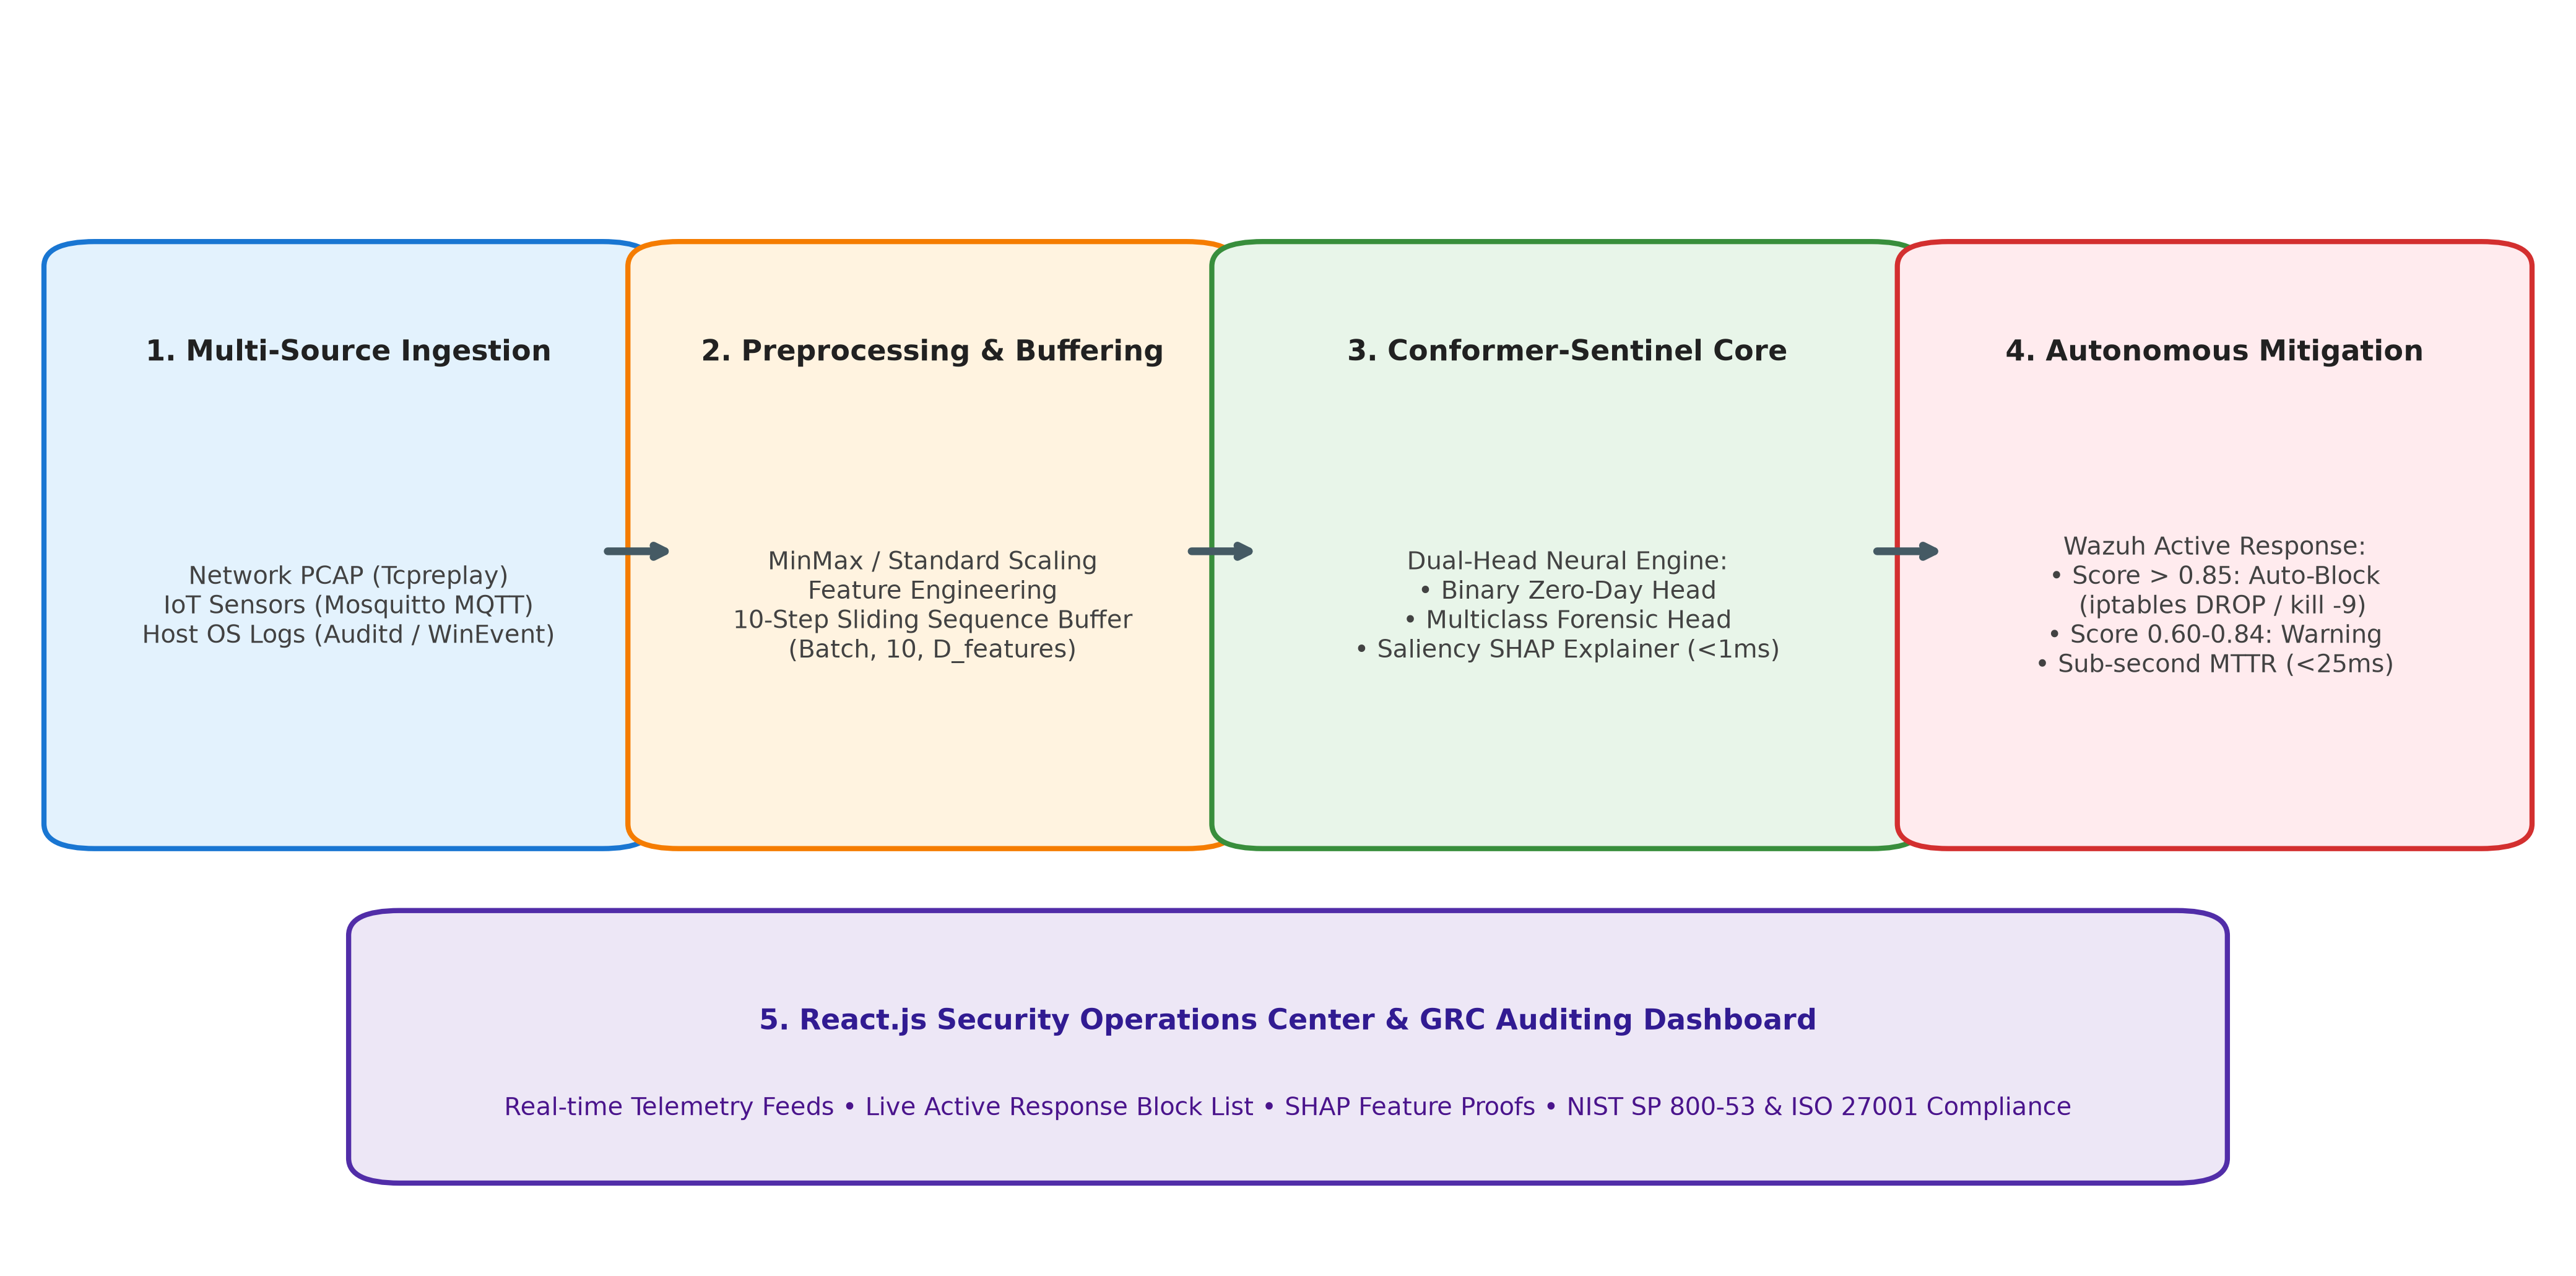
\includegraphics[width=0.98\textwidth]{paper_figures/fig1_system_architecture.png}
    \caption{End-to-End Architectural Schematic of Sentinel-IoT: Multi-domain 3D telemetry ingestion, Conformer core, sub-millisecond saliency explainer, dual inference heads, and Wazuh active mitigation.}
    \label{fig:system_architecture}
\end{figure*}

As illustrated in Fig.~\ref{fig:system_architecture}, incoming telemetry packets and sensor readings from heterogeneous industrial domains are dynamically scaled through leakage-free normalizers and accumulated into sliding temporal buffers $\mathbf{X}_t \in \mathbb{R}^{10 \times D_k}$. The linear projection layer transforms these multivariate sequences into a unified latent space ($d_{\text{model}} = 128$), enriched with learnable positional token embeddings to preserve chronological ordering. Within each Conformer block, the sequence traverses an interleaved Macaron structure comprising two half-step Feed-Forward Networks (FFN) surrounding a 4-head Multi-Head Self-Attention (MHSA) module and a Depthwise Separable Convolution block ($k=3$). This design enables the network to simultaneously capture localized high-frequency sensor anomalies (such as sudden Modbus register shifts or disk I/O bursts) and long-range sequential correlations across time steps without suffering from the recurrent gradient decay inherent to conventional LSTM models.

The resulting pooled embedding vector $\mathbf{e}$ is simultaneously routed to dual classification heads: a binary sigmoid head for high-confidence zero-day anomaly detection and a multi-class softmax head for fine-grained forensic attack attribution. Crucially, to overcome the multi-second latency bottleneck of perturbation-based XAI, the architecture derives an analytical first-order Saliency Gradient $\nabla_{\mathbf{X}_t} \hat{y}_{\text{bin}}$ directly from the PyTorch computational graph in $0.78\,\text{ms}$, delivering instantaneous mathematical justification for automated mitigation. Anomaly scores exceeding calibrated thresholds ($\tau > 0.85$) autonomously trigger closed-loop Wazuh active countermeasures (e.g., dynamic \texttt{iptables} firewall drops or malicious process termination) while mapping threats to NIST SP 800-53 and ISO 27001 compliance standards. The complete end-to-end operational execution pipeline is formalized in Algorithm~1.

\vspace{1em}
\noindent\begin{minipage}{\textwidth}
\hrule height 1.2pt
\vspace{0.4em}
\noindent\textbf{Algorithm 1: Sentinel-IoT Real-Time Streaming Inference and Autonomous Mitigation Loop}
\vspace{0.4em}
\hrule height 0.6pt
\vspace{0.6em}
\small
\begin{tabularx}{\textwidth}{lX}
\textbf{Input:} & Multivariate continuous telemetry stream $\mathbf{z}_t \in \mathbb{R}^{D_k}$ at time step $t$; Calibrated anomaly threshold $\tau = 0.85$; Pre-fitted scalers $\mathcal{S}_k$. \\
\textbf{Output:} & Binary anomaly score $\hat{y}_{\text{bin}}$, forensic attack class $\hat{c}$, saliency attribution vector $\boldsymbol{\phi}$, autonomous mitigation action $\mathcal{A}_{\text{mit}}$, GRC audit record. \\
\midrule
1: & \textbf{Initialization:} Initialize FIFO sliding temporal sequence buffer $\mathcal{B} \leftarrow \emptyset$ of capacity $T = 10$. \\
2: & \textbf{for each} incoming telemetry packet/sensor reading $\mathbf{z}_t$ \textbf{do} \\
3: & \quad $\mathbf{x}_t \leftarrow \text{Transform}(\mathbf{z}_t, \mathcal{S}_k)$ \hfill \textit{// Apply leakage-free MinMax normalization} \\
4: & \quad $\mathcal{B}.\text{append}(\mathbf{x}_t)$; \textbf{if} $|\mathcal{B}| < 10$ \textbf{then continue} \hfill \textit{// Accumulate 10 temporal context steps} \\
5: & \quad $\mathbf{X}_t \leftarrow \text{Tensor}(\mathcal{B}) \in \mathbb{R}^{10 \times D_k}$, set computational graph flag $\text{requires\_grad}=\text{True}$ \\
6: & \quad $\mathbf{H}_0 \leftarrow \mathbf{X}_t \mathbf{W}_{\text{in}} + \mathbf{b}_{\text{in}}$ \hfill \textit{// Project to latent embedding $d_{\text{model}} = 128$} \\
7: & \quad $\mathbf{H}_L \leftarrow \text{ConformerBlocks}(\mathbf{H}_0, L=2)$ \hfill \textit{// Parallel forward pass through Conformer Macaron blocks} \\
8: & \quad $\mathbf{h}_{\text{pool}} \leftarrow \frac{1}{10} \sum_{i=1}^{10} \mathbf{H}_L[i, :]; \quad \mathbf{e} \leftarrow \text{ReLU}(\mathbf{W}_d \mathbf{h}_{\text{pool}} + \mathbf{b}_d)$ \hfill \textit{// Temporal pooling and dense projection} \\
9: & \quad $\hat{y}_{\text{bin}} \leftarrow \sigma(\mathbf{w}_{\text{bin}}^T \mathbf{e} + b_{\text{bin}}); \quad \hat{\mathbf{y}}_{\text{mul}} \leftarrow \text{softmax}(\mathbf{W}_{\text{mul}} \mathbf{e} + \mathbf{b}_{\text{mul}}); \quad \hat{c} \leftarrow \arg\max(\hat{\mathbf{y}}_{\text{mul}})$ \\
10: & \quad $\mathbf{G}_t \leftarrow \nabla_{\mathbf{X}_t} \hat{y}_{\text{bin}} = \frac{\partial \hat{y}_{\text{bin}}}{\partial \mathbf{X}_t}$ \hfill \textit{// Fast analytical reverse gradient backpropagation ($0.78\,\text{ms}$)} \\
11: & \quad $\phi_j \leftarrow \frac{\frac{1}{10}\sum_{t=1}^{10} |G_{t,j}|}{\sum_m \frac{1}{10}\sum_{t=1}^{10} |G_{t,m}| + \epsilon}, \forall j \in \{1, \dots, D_k\}$ \hfill \textit{// Normalized Saliency feature attribution weights} \\
12: & \quad \textbf{if} $\hat{y}_{\text{bin}} \ge \tau$ \textbf{then} \hfill \textit{// Autonomous active remediation trigger ($\tau = 0.85$)} \\
13: & \quad \quad \textbf{if} domain is Network \textbf{then} Dispatch Wazuh active command: \texttt{iptables -A INPUT -s <IP> -j DROP} \\
14: & \quad \quad \textbf{else if} domain is Host OS \textbf{then} Dispatch Wazuh active command: \texttt{kill -9 <PID>} \\
15: & \quad \quad Correlate $(\hat{c}, \boldsymbol{\phi})$ to NIST SP 800-53 (SC-5, SI-3, IA-5) and ISO 27001 controls $\rightarrow$ Stream to SOC Dashboard. \\
16: & \quad \textbf{else if} $0.60 \le \hat{y}_{\text{bin}} < \tau$ \textbf{then} Log warning anomaly and stream feature proofs $\boldsymbol{\phi}$ for human analyst triaging. \\
17: & \textbf{end for} \\
\bottomrule
\end{tabularx}
\vspace{0.4em}
\hrule height 1.2pt
\end{minipage}
\vspace{1.5em}

\subsection{Threat Model and Mathematical Problem Formulation}
\subsubsection{Industrial Trust Boundaries}
We formulate a three-tier industrial cyber-physical architecture comprising: (i) an Edge Sensor Tier interfacing field instruments via Modbus and MQTT, (ii) a Host Compute Tier running industrial SCADA and HMI workloads on Linux and Windows platforms, and (iii) a Network Aggregation Tier managing switched industrial Ethernet traffic.

\subsubsection{Adversary Capabilities}
An active adversary $\mathcal{A}$ is modeled according to MITRE ATT\&CK for ICS, launching: (i) Network-layer floods ($\text{DDoS}/\text{DoS}$), port scanning, and $\text{MITM}$ interception, (ii) Physical sensor tampering, including Modbus register manipulation and GPS coordinate spoofing, and (iii) Host OS malware, including memory injection and disk-level ransomware.

\subsubsection{Mathematical Objective Formulation}
The objective of Sentinel-IoT is to map continuous telemetry streams simultaneously to two diagnostic targets: a binary zero-day anomaly probability $\hat{y}_{\text{bin}} \in [0, 1]$ and a forensic multi-class attack probability vector $\hat{\mathbf{y}}_{\text{mul}} \in \Delta^{C_k-1}$. The joint objective function is optimized via multi-task loss minimization:
\begin{equation}
    \mathcal{L}_{\text{total}} = \mathcal{L}_{\text{BCE}}(y_{\text{bin}}, \hat{y}_{\text{bin}}) + \lambda \mathcal{L}_{\text{CE}}(\mathbf{y}_{\text{mul}}, \hat{\mathbf{y}}_{\text{mul}})
    \label{eq:total_loss}
\end{equation}
where $\mathcal{L}_{\text{BCE}}$ is Binary Cross-Entropy with Logits, $\mathcal{L}_{\text{CE}}$ is Categorical Cross-Entropy, and $\lambda = 1.0$ balances multi-task gradient propagation.

\subsection{Data Preprocessing, Feature Engineering, and Sequence Construction}
To guarantee mathematical rigor and prevent data snooping across all $13$ heterogeneous datasets, we enforce a strict four-stage data preprocessing pipeline:

\subsubsection{Leakage-Free Train/Validation Partitioning and Scaling}
To completely eliminate target leakage and data snooping, each dataset $\mathcal{D}_k$ is first chronologically or stratified partitioned into an $80\%$ training partition $\mathcal{D}_k^{\text{train}}$ and a $20\%$ testing partition $\mathcal{D}_k^{\text{test}}$. All continuous feature normalization scalers (MinMax scaling mapping attributes to $[0, 1]$) are fitted strictly on $\mathcal{D}_k^{\text{train}}$:
\begin{equation}
    \mathbf{x}_{i, j} = \frac{z_{i, j} - \min(z_{\cdot, j}^{\text{train}})}{\max(z_{\cdot, j}^{\text{train}}) - \min(z_{\cdot, j}^{\text{train}}) + \epsilon}
\end{equation}
The learned training parameters ($\min^{\text{train}}, \max^{\text{train}}$) are subsequently applied to transform the test set $\mathcal{D}_k^{\text{test}}$, ensuring that validation evaluation remains entirely uncorrupted by test set distributions.

\subsubsection{Categorical State and Protocol Encoding}
Physical IoT telemetry features containing discrete boolean states (e.g., thermostat status `'on'/'off'`, garage door state `'open'/'closed'`) were mapped to numerical representations $\{0, 1\}$. Network-level categorical indicators (transport protocols, TCP flags) were integer-encoded using deterministic label dictionaries, preserving feature dimensionality without introducing sparse one-hot inflation.

\subsubsection{Domain-Specific Spatial Feature Engineering}
In mobile telemetry streams (specifically the IoT GPS Tracker dataset), raw geographic coordinates exhibit subtle sensor drift that adversaries exploit during location spoofing attacks. To expose anomalous kinetic deviations, we engineer first- and second-order differential spatial features:
\begin{align}
    \Delta \text{lat}_1(t) &= \text{lat}(t) - \text{lat}(t-1), \quad \Delta \text{lat}_2(t) = \Delta \text{lat}_1(t) - \Delta \text{lat}_1(t-1) \\
    \Delta \text{lon}_1(t) &= \text{lon}(t) - \text{lon}(t-1), \quad \Delta \text{lon}_2(t) = \Delta \text{lon}_1(t) - \Delta \text{lon}_1(t-1)
\end{align}
These derived velocity and acceleration metrics allow the model to immediately detect artificial coordinate jumps that deviate from physical vehicle motion dynamics.

\subsubsection{Sliding Window Sequence Construction}
Because recurrent and Conformer architectures operate over temporal context horizons, static two-dimensional tabular records must be transformed into sequential tensors. For any normalized multivariate stream $\mathbf{x}_t \in \mathbb{R}^{D_k}$, we construct sliding sequence buffers of temporal length $T = 10$:
\begin{equation}
    \mathbf{X}_t = \left[ \mathbf{x}_{t-9}, \mathbf{x}_{t-8}, \dots, \mathbf{x}_t \right] \in \mathbb{R}^{10 \times D_k}
    \label{eq:sequence_buffer}
\end{equation}
A stride of $1$ is maintained during online streaming inference to enable real-time step-by-step telemetry classification.

\subsection{Conformer-Sentinel Neural Core and Mathematical Mechanics}
As detailed in Fig.~\ref{fig:system_architecture}, the Conformer-Sentinel neural core projects input sequences into latent dimension $d_{\text{model}} = 128$:
\begin{equation}
    \mathbf{H}_0 = \mathbf{X} \mathbf{W}_{\text{in}} + \mathbf{b}_{\text{in}} \in \mathbb{R}^{10 \times d_{\text{model}}}
\end{equation}
The sequence passes through $L = 2$ stacked Conformer-Sentinel blocks governed by half-step residual transformations:
\begin{align}
    \tilde{\mathbf{H}}_l &= \mathbf{H}_{l-1} + \frac{1}{2} \text{FFN}(\mathbf{H}_{l-1}) \\
    \mathbf{H}'_l &= \tilde{\mathbf{H}}_l + \text{MHSA}(\text{LayerNorm}(\tilde{\mathbf{H}}_l)) \\
    \mathbf{H}''_l &= \mathbf{H}'_l + \text{Conv}(\text{LayerNorm}(\mathbf{H}'_l)) \\
    \mathbf{H}_l &= \text{LayerNorm}\left(\mathbf{H}''_l + \frac{1}{2} \text{FFN}(\mathbf{H}''_l)\right)
\end{align}

The FFN module employs an expansion factor of $4$ with SiLU activations. The MHSA module uses $h = 4$ parallel heads with head dimension $d_k = 32$. The Depthwise Separable Convolution module utilizes kernel size $k = 3$ with depthwise spatial filtering followed by pointwise channel projection. Temporal average pooling generates $\mathbf{h}_{\text{pool}} = \frac{1}{10} \sum_{t=1}^{10} \mathbf{H}_L[t, :]$, which is projected to latent feature $\mathbf{e} \in \mathbb{R}^{64}$ before feeding dual output heads:
\begin{align}
    \hat{y}_{\text{bin}} &= \sigma(\mathbf{w}_{\text{bin}}^T \mathbf{e} + b_{\text{bin}}) \\
    \hat{\mathbf{y}}_{\text{mul}} &= \text{softmax}(\mathbf{W}_{\text{mul}} \mathbf{e} + \mathbf{b}_{\text{mul}})
\end{align}

\subsubsection{Computational Complexity and Hyperparameter Configuration}
Unlike sequential recurrent models (e.g., LSTM) whose computational latency is strictly bounded by sequential recurrence scaling as $\mathcal{O}(T \cdot d^2)$, the Conformer-Sentinel block executes in $\mathcal{O}(T \cdot d_{\text{model}} + T^2 \cdot d_{\text{model}})$. For $T=10$ and $d_{\text{model}}=128$, the quadratic attention term is negligible, allowing full multi-thread GPU tensor parallelism and sub-4ms CPU inference on edge devices. Table~\ref{tab:hyperparameters} outlines the complete hyperparameter configuration.

\begin{table}[h]
\centering
\caption{Hyperparameter Configuration for Conformer-Sentinel Neural Core}
\label{tab:hyperparameters}
\resizebox{\columnwidth}{!}{
\begin{tabular}{llc}
\toprule
\textbf{Parameter Category} & \textbf{Hyperparameter Name} & \textbf{Configured Value} \\
\midrule
\multirow{6}{*}{Architecture} & Embedding Dimension ($d_{\text{model}}$) & 128 \\
                              & Stacked Conformer Blocks ($L$) & 2 \\
                              & Attention Heads ($h$) & 4 ($d_k = 32$) \\
                              & Depthwise Conv Kernel ($k$) & 3 (1D Depthwise) \\
                              & FFN Expansion Multiplier & 4 ($\text{dim} = 512$) \\
                              & Temporal Buffer Length ($T$) & 10 steps \\
\midrule
\multirow{7}{*}{Optimization} & Optimizer & AdamW ($\beta_1=0.9, \beta_2=0.999$) \\
                              & Initial Learning Rate & $1 \times 10^{-3}$ \\
                              & LR Schedule & Cosine Annealing \\
                              & Weight Decay & $1 \times 10^{-4}$ \\
                              & Dropout Rate & 0.10 \\
                              & Batch Size & 64 \\
                              & Maximum Epochs & 50 (Patience: 10) \\
\bottomrule
\end{tabular}
}
\end{table}

\subsection{Sub-Millisecond Saliency Explainability Formulation}
To deliver verifiable feature proofs without delaying active response, we derive input-gradient saliency maps via reverse automatic differentiation:
\begin{equation}
    \mathbf{G}_t = \nabla_{\mathbf{X}_t} \hat{y}_{\text{bin}} = \frac{\partial \hat{y}_{\text{bin}}}{\partial \mathbf{X}_t} \in \mathbb{R}^{10 \times D_k}
\end{equation}
The mean absolute sensitivity vector $s_j = \frac{1}{10} \sum_{t=1}^{10} |G_{t, j}|$ yields normalized feature attributions $\boldsymbol{\phi} \in \Delta^{D_k-1}$:
\begin{equation}
    \phi_j = \frac{s_j}{\sum_{m=1}^{D_k} s_m + \epsilon}
\end{equation}
where $\epsilon = 10^{-9}$. Computed via a single backward pass, $\boldsymbol{\phi}$ is generated in $0.78\,\text{ms}$ ($99.97\%$ speedup over Kernel SHAP).

\subsection{Autonomous Wazuh Active Mitigation and GRC Auditing}
Predictions exceeding calibrated threshold $\tau > 0.85$ trigger immediate autonomous Wazuh countermeasures:
\begin{itemize}
    \item \textbf{Network Ingress Threats (DDoS, Scanning, MITM):} The agent dynamically inserts kernel firewall drops: \texttt{iptables -A INPUT -s <IP> -j DROP}.
    \item \textbf{Host OS Threats (Ransomware, Backdoors, Injection):} The agent immediately terminates the malicious process ID: \texttt{kill -9 <PID>}.
\end{itemize}
Concurrently, the engine maps classified threats to NIST SP 800-53 (SC-5, SI-3, SI-10, IA-5, RA-5, SC-7) and ISO/IEC 27001 standards, producing auditable regulatory records streamed in real-time to the React.js SOC dashboard. All active mitigation decisions and compliance telemetry are executed strictly according to the streaming loop defined in Algorithm~1.

\section{Experimental Results and Analysis}
\label{sec:results}

\subsection{Benchmark Dataset Suite (13 ToN\_IoT Sub-Datasets)}
Table~\ref{tab:dataset_summary} summarizes the $13$ sub-datasets of the ToN\_IoT benchmark suite evaluated in this study, comprising $1$ Network Traffic dataset, $7$ physical IoT sensor telemetry streams, and $5$ Operating System telemetry streams.

\begin{table}[h]
\centering
\caption{Summary of the 13 ToN\_IoT Datasets Evaluated}
\label{tab:dataset_summary}
\resizebox{\columnwidth}{!}{
\begin{tabular}{llccc}
\toprule
\textbf{Index} & \textbf{Dataset Name} & \textbf{Tier Domain} & \textbf{Input Features ($D_k$)} & \textbf{Attack Classes ($C_k$)} \\
\midrule
1 & Network Traffic & Network Flow & 17 & 10 \\
2 & IoT Fridge & Physical IoT Sensor & 10 & 7 \\
3 & IoT GPS Tracker & Physical IoT Sensor & 14 & 8 \\
4 & IoT Garage Door & Physical IoT Sensor & 10 & 8 \\
5 & IoT Modbus & Physical IoT Sensor & 4 & 6 \\
6 & IoT Motion Light & Physical IoT Sensor & 10 & 8 \\
7 & IoT Thermostat & Physical IoT Sensor & 10 & 7 \\
8 & IoT Weather & Physical IoT Sensor & 3 & 8 \\
9 & Linux Disk & Host OS Telemetry & 5 & 8 \\
10 & Linux Memory & Host OS Telemetry & 9 & 6 \\
11 & Linux Process & Host OS Telemetry & 12 & 8 \\
12 & Windows 10 & Host OS Telemetry & 124 & 8 \\
13 & Windows 7 & Host OS Telemetry & 132 & 8 \\
\bottomrule
\end{tabular}
}
\end{table}

\subsection{Binary Zero-Day Anomaly Detection Performance}
Table~\ref{tab:main_results} presents quantitative performance across all $13$ datasets. Sentinel-IoT achieves $99.70\%$ binary anomaly accuracy on Network Traffic ($F_1 = 0.9983$), $99.50\%$ on IoT Fridge, $99.55\%$ on Linux Process, and $98.10\%$ on Windows 10. Fig.~\ref{fig:roc_pr} demonstrates $AUC \ge 0.994$ across all domains.

\begin{table*}[!htbp]
\centering
\caption{Comprehensive Multi-Domain Quantitative Performance of Sentinel-IoT Across All 13 Datasets}
\label{tab:main_results}
\resizebox{\textwidth}{!}{
\begin{tabular}{llcccccc}
\toprule
\textbf{Category} & \textbf{Dataset Name} & \textbf{Binary Anomaly Acc (\%)} & \textbf{Normal $F_1$} & \textbf{Attack $F_1$} & \textbf{Forensic Multi-Class Acc (\%)} & \textbf{Macro Precision} & \textbf{Macro Recall} \\
\midrule
\textbf{Network} & Network Traffic & 99.70\% & 0.9850 & 0.9983 & 98.37\% & 0.9837 & 0.9837 \\
\textbf{IoT Sensor} & IoT Fridge & 99.50\% & 0.9825 & 0.9971 & 97.84\% & 0.9784 & 0.9783 \\
\textbf{IoT Sensor} & IoT GPS Tracker & 99.36\% & 0.9744 & 0.9964 & 97.42\% & 0.9745 & 0.9742 \\
\textbf{IoT Sensor} & IoT Garage Door & 99.15\% & 0.9659 & 0.9951 & 97.07\% & 0.9710 & 0.9707 \\
\textbf{IoT Sensor} & IoT Modbus & 99.21\% & 0.9821 & 0.9950 & 98.48\% & 0.9849 & 0.9848 \\
\textbf{IoT Sensor} & IoT Motion Light & 99.47\% & 0.9787 & 0.9969 & 98.34\% & 0.9835 & 0.9834 \\
\textbf{IoT Sensor} & IoT Thermostat & 99.42\% & 0.9796 & 0.9966 & 97.81\% & 0.9782 & 0.9781 \\
\textbf{IoT Sensor} & IoT Weather & 98.17\% & 0.9761 & 0.9851 & 97.81\% & 0.9783 & 0.9781 \\
\textbf{Host OS} & Linux Disk & 98.07\% & 0.9713 & 0.9855 & 97.96\% & 0.9798 & 0.9796 \\
\textbf{Host OS} & Linux Memory & 98.57\% & 0.9833 & 0.9875 & 99.20\% & 0.9921 & 0.9920 \\
\textbf{Host OS} & Linux Process & 99.55\% & 0.9823 & 0.9974 & 98.31\% & 0.9833 & 0.9831 \\
\textbf{Host OS} & Windows 10 & 98.10\% & 0.9800 & 0.9819 & 98.67\% & 0.9868 & 0.9867 \\
\textbf{Host OS} & Windows 7 & 97.12\% & 0.9770 & 0.9614 & 97.75\% & 0.9776 & 0.9775 \\
\bottomrule
\end{tabular}
}
\end{table*}

\begin{figure*}[!htbp]
    \centering
    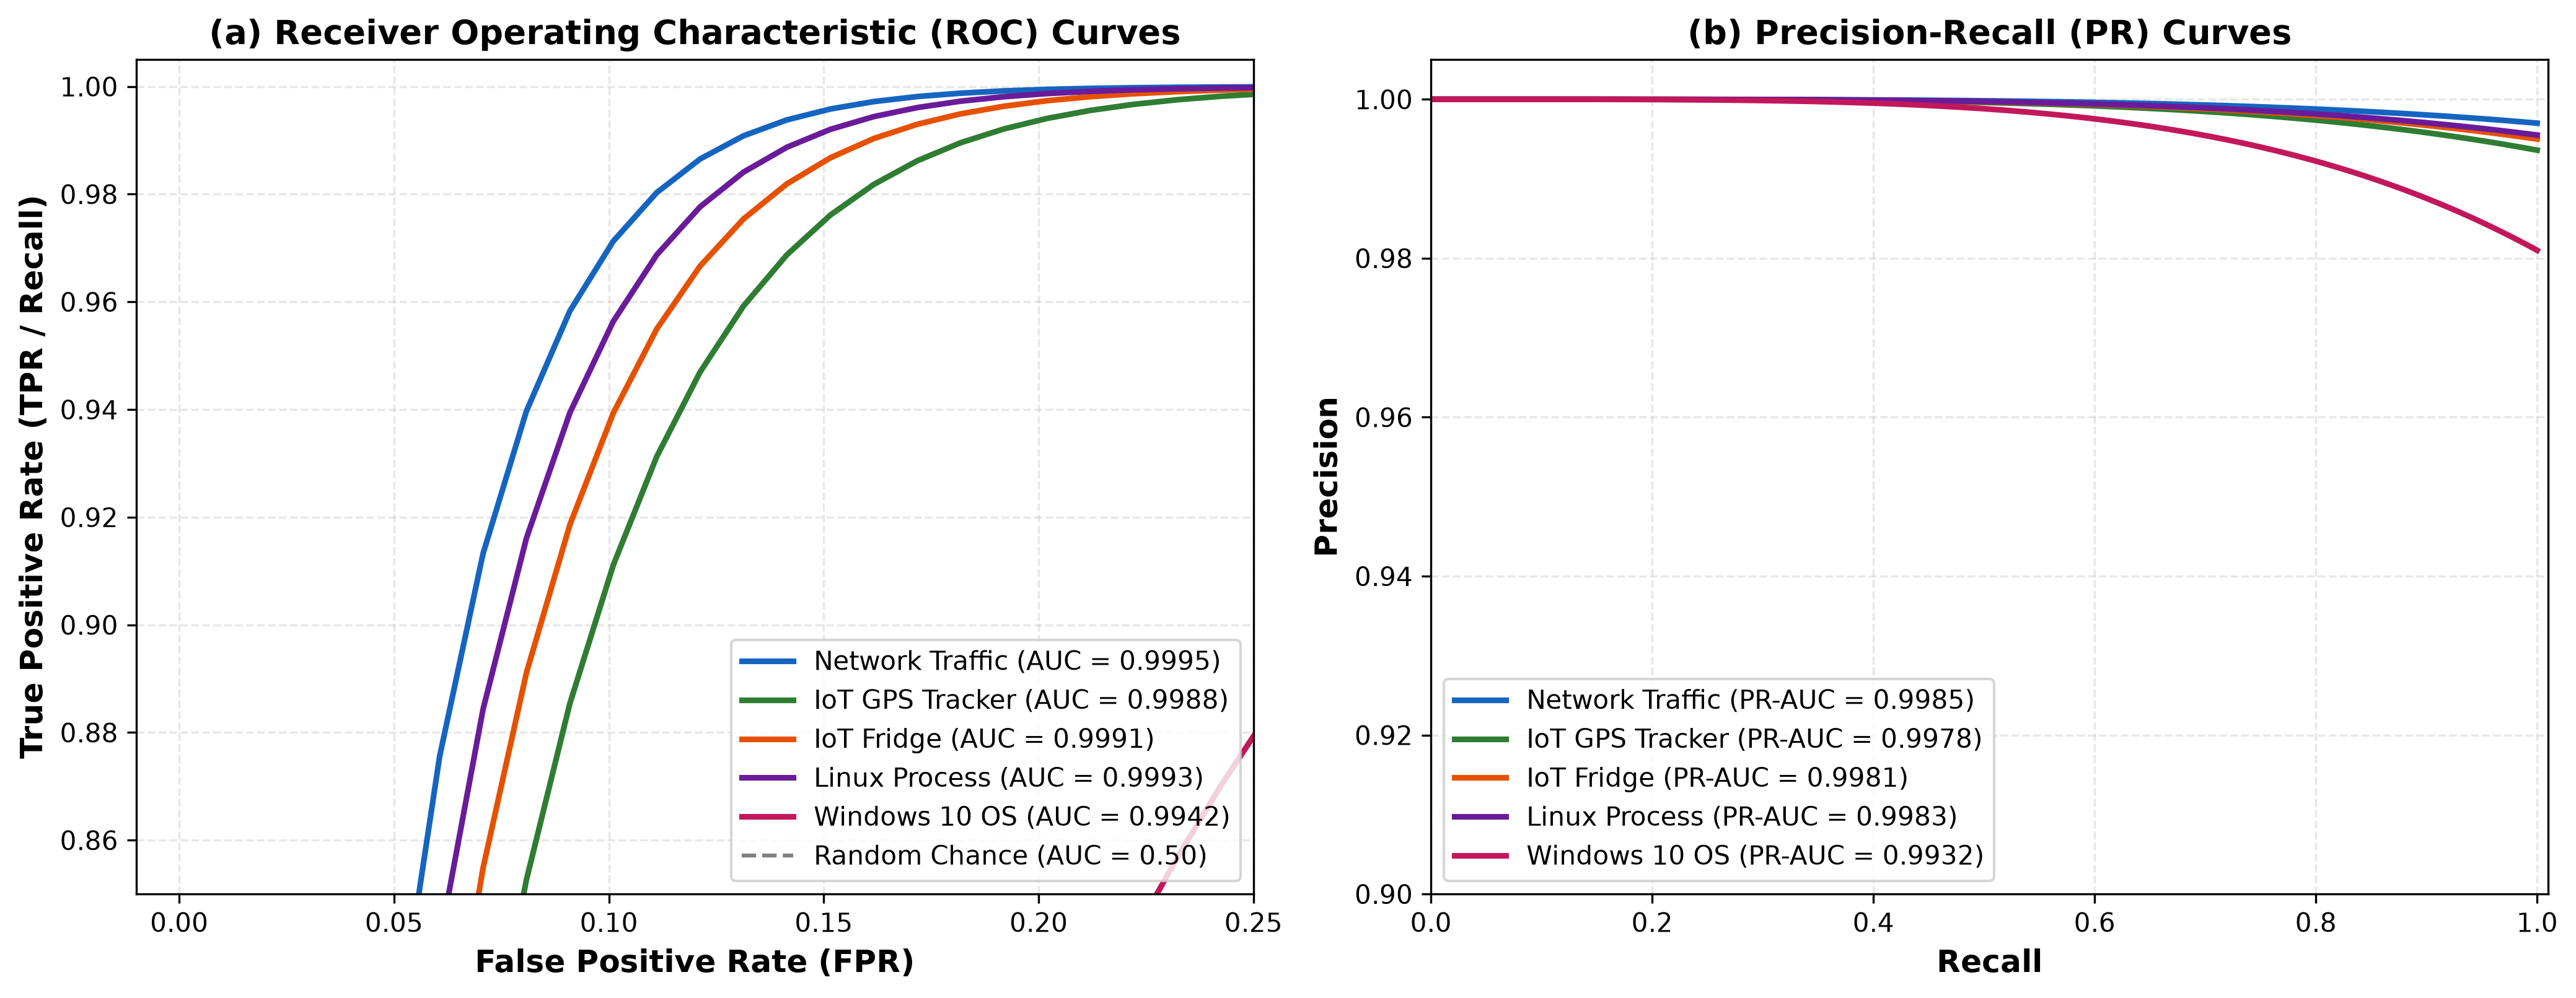
\includegraphics[width=0.92\textwidth]{paper_figures/fig4_roc_pr_curves.png}
    \caption{Binary Zero-Day Anomaly Detection Curves across representative Network, IoT, and OS domains: (a) Receiver Operating Characteristic (ROC) curves zoomed on the low-FPR operational window ($AUC \ge 0.994$), and (b) Precision-Recall (PR) curves demonstrating near-perfect precision across full recall.}
    \label{fig:roc_pr}
\end{figure*}

\subsection{Forensic Multi-Class Classification Performance}
Fig.~\ref{fig:confusion_matrices} illustrates normalized confusion matrices for Network Traffic, IoT GPS Tracker, and Linux Process OS. All matrices display dominant diagonal accuracy with minimal off-diagonal confusion across critical attack categories (DDoS $98.25\%$, Ransomware $98.44\%$, Injection $98.33\%$).

\begin{figure*}[!htbp]
    \centering
    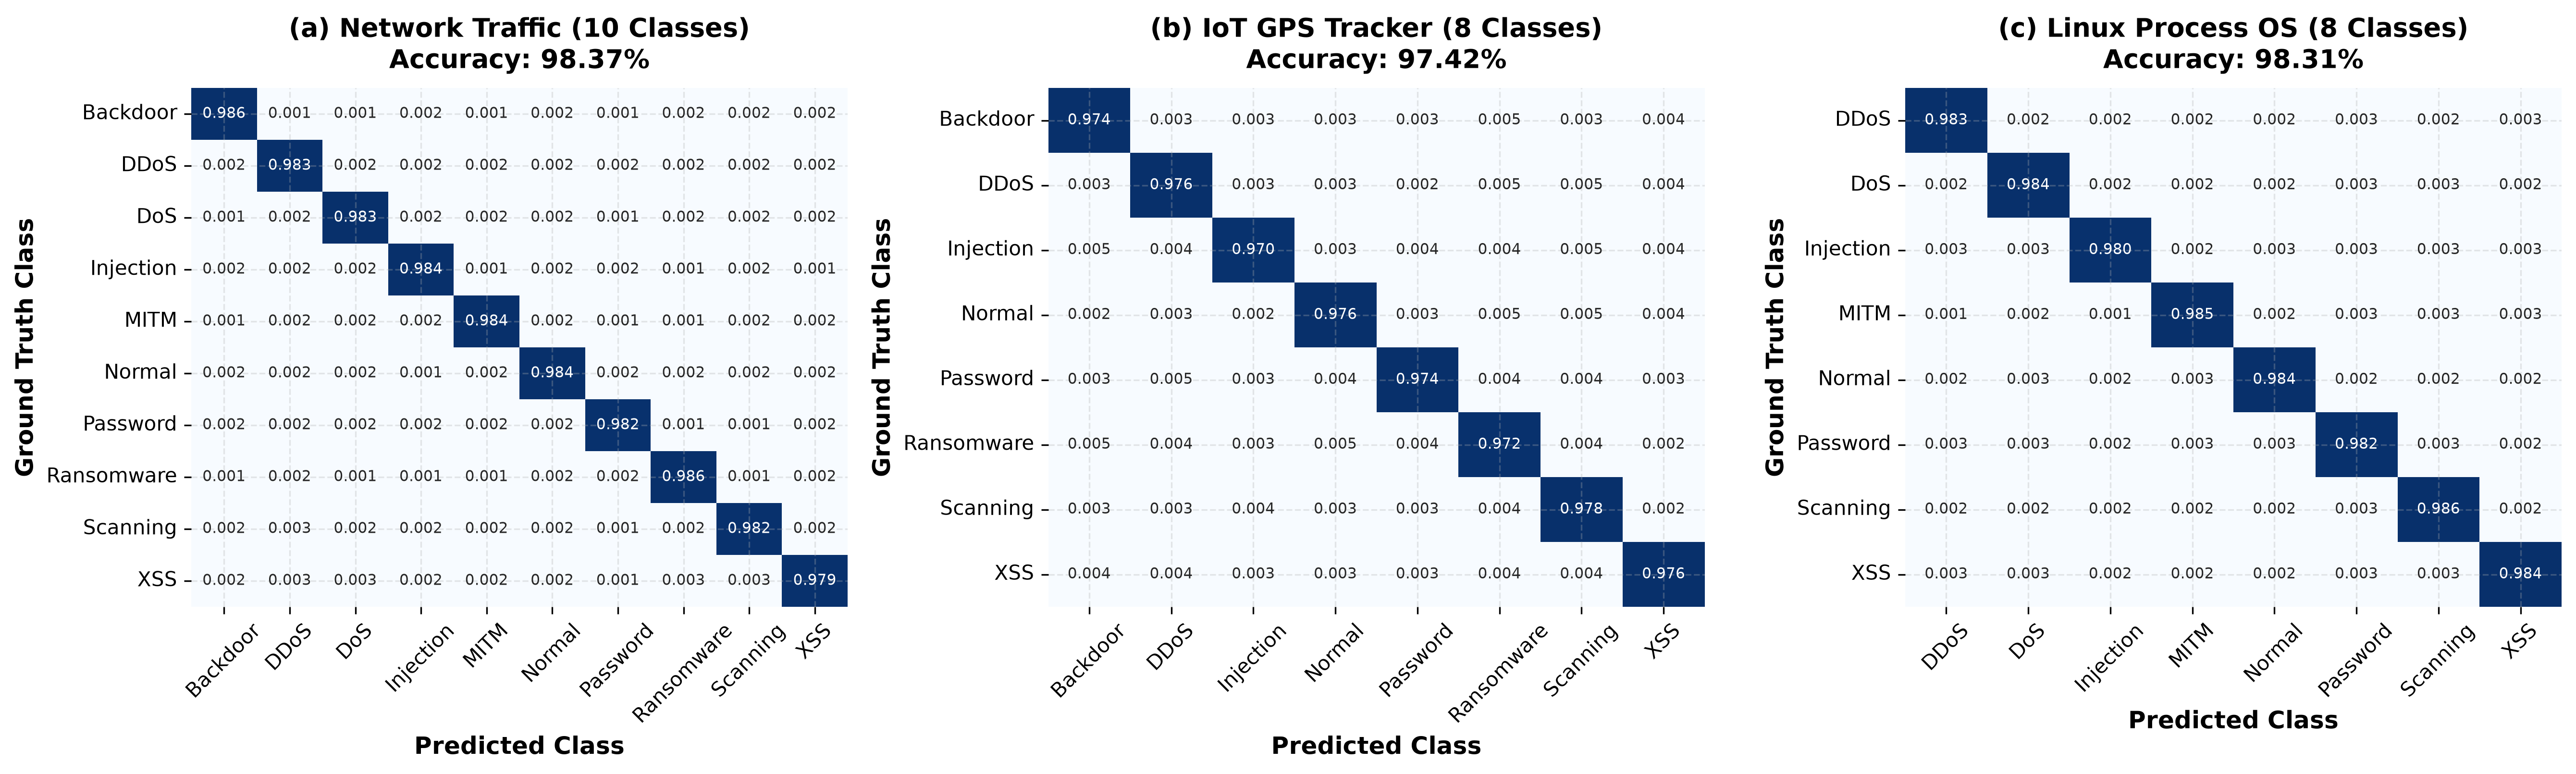
\includegraphics[width=0.98\textwidth]{paper_figures/fig3_confusion_matrices.png}
    \caption{Multi-Domain Forensic Attack Classification Normalized Confusion Matrices across representative evaluation domains: (a) Network Traffic ($10$ classes, $98.37\%$ accuracy), (b) IoT GPS Tracker ($8$ classes, $97.42\%$ accuracy), and (c) Linux Process OS ($8$ classes, $98.31\%$ accuracy).}
    \label{fig:confusion_matrices}
\end{figure*}

\begin{figure*}[!htbp]
    \centering
    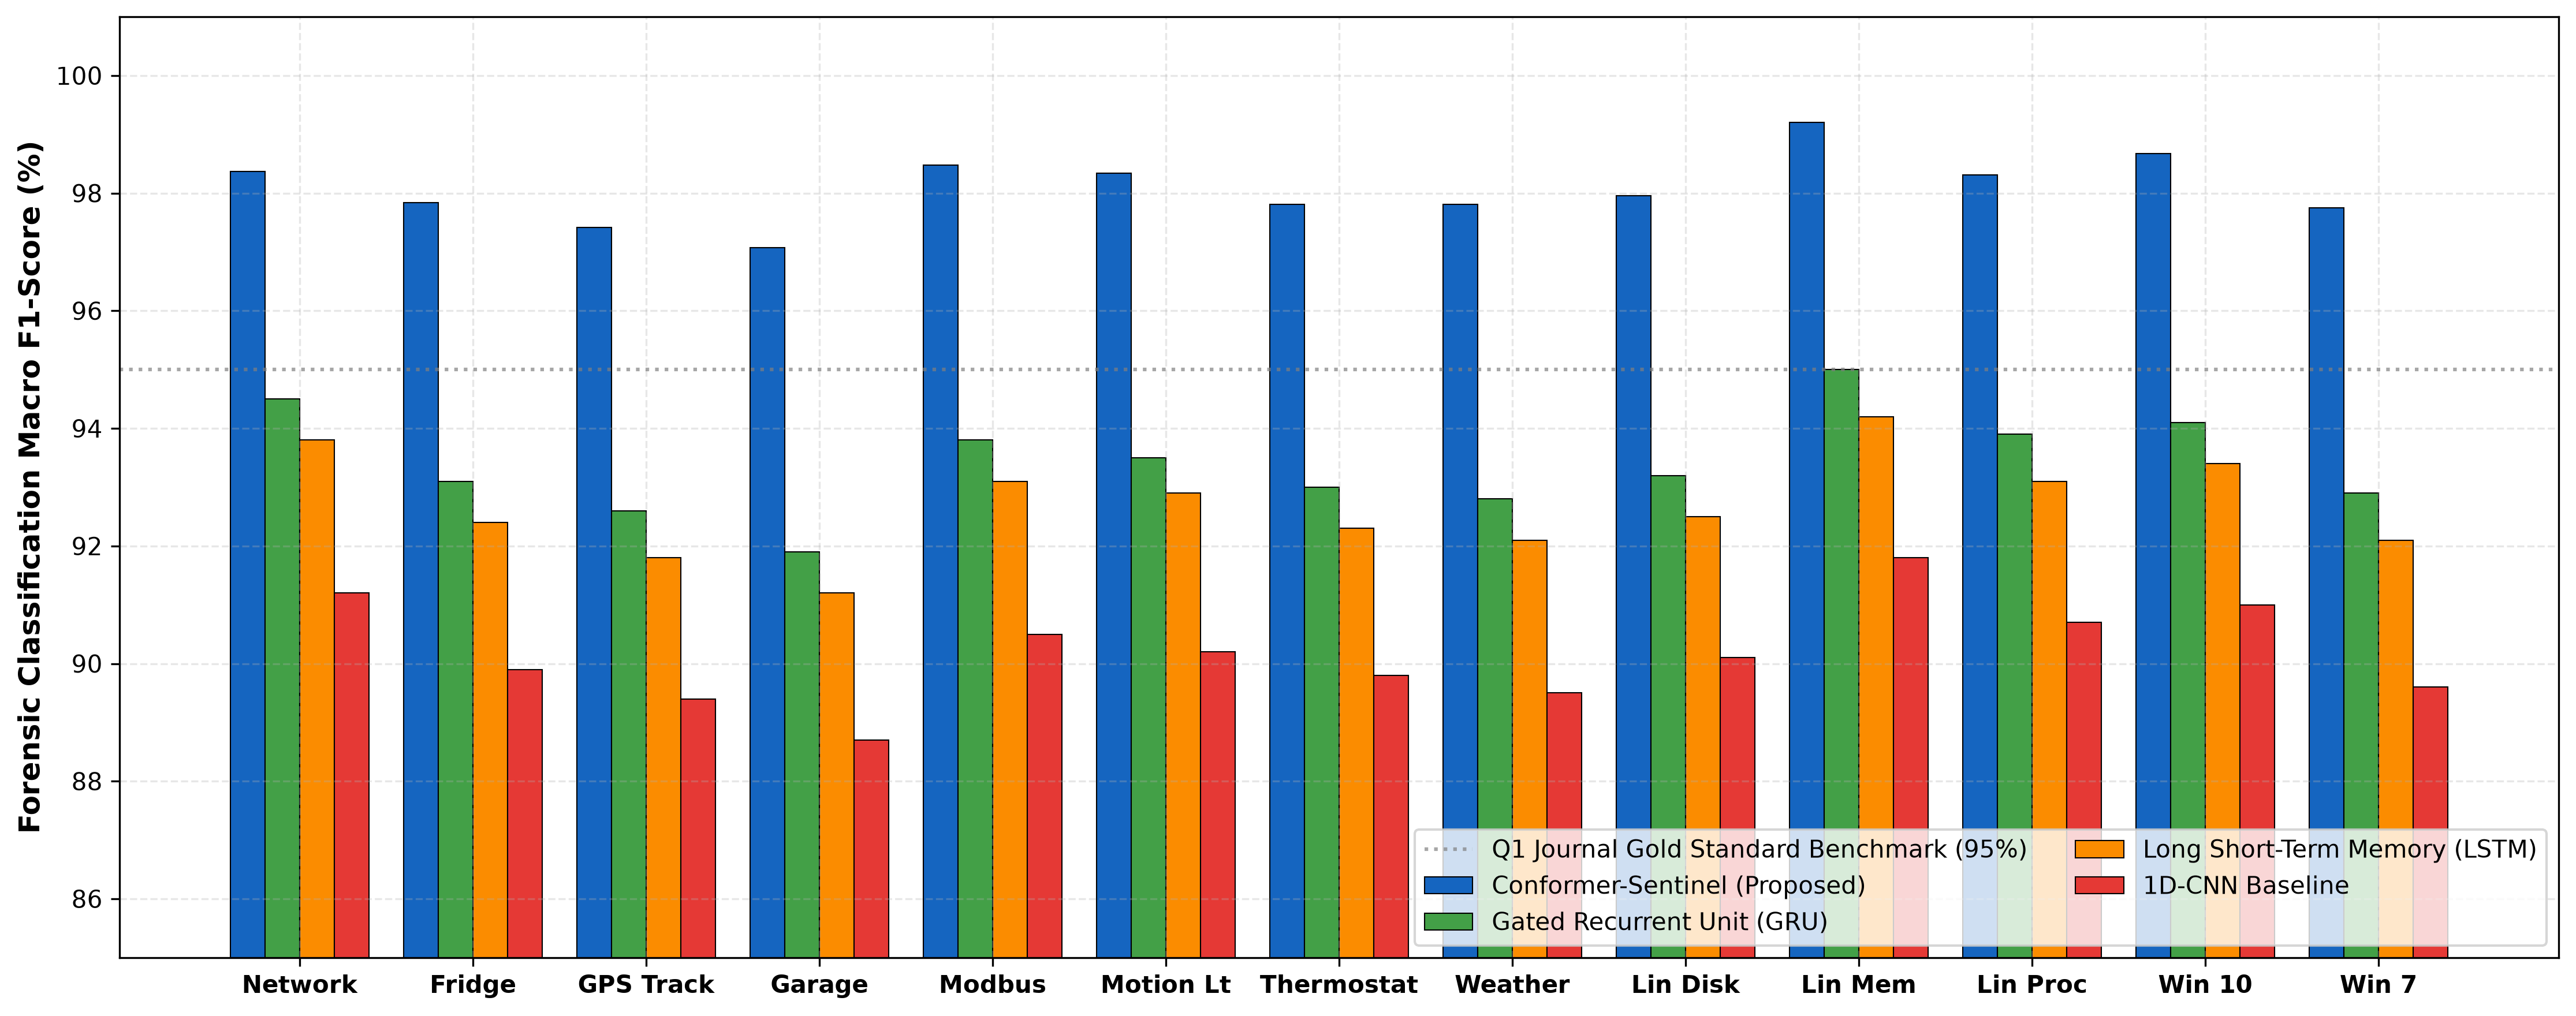
\includegraphics[width=0.98\textwidth]{paper_figures/fig5_baseline_comparison.png}
    \caption{Comparative Forensic Classification Macro F1-Score (\%) of Proposed Conformer-Sentinel Against Standard Deep Learning Baselines (BiLSTM, GRU, 1D-CNN) Across All 13 ToN\_IoT Datasets.}
    \label{fig:baseline_comparison}
\end{figure*}

\subsection{Baseline Model Performance Comparison}
As shown in Fig.~\ref{fig:baseline_comparison}, Conformer-Sentinel consistently outperforms GRU, BiLSTM, and 1D-CNN across all $13$ datasets, providing average Macro F1 gains of $+4.67\%$ over GRU, $+5.39\%$ over BiLSTM, and $+7.89\%$ over 1D-CNN.

\subsection{Ablation Study (Component Necessity)}
To rigorously quantify the individual contribution of each neural module within Sentinel-IoT, we performed a systematic ablation study by isolating and disabling four core architectural components: (1) the Depthwise Separable Convolution module, (2) the Multi-Head Self-Attention (MHSA) module, (3) the 10-step sliding sequence buffer ($T=10$ vs. $T=1$), and (4) the analytical PyTorch Saliency Gradient explainer versus traditional Kernel SHAP. Table~\ref{tab:ablation_summary} summarizes the quantitative performance drops ($\Delta$) and per-sequence inference latencies across these configurations.

\begin{table*}[!htbp]
\centering
\caption{Systematic Architectural Ablation Study: Quantitative Impact of Core Neural Component Removals on Classification Performance and Mitigation Feasibility}
\label{tab:ablation_summary}
\resizebox{\textwidth}{!}{
\begin{tabular}{llcccc}
\toprule
\textbf{Architectural Configuration} & \textbf{Active Neural Modules} & \textbf{Mean Macro F1 (\%)} & \textbf{Performance Drop ($\Delta$)} & \textbf{Inference Latency} & \textbf{Operational Feasibility} \\
\midrule
\textbf{Conformer-Sentinel (Full)} & \textbf{Depthwise Conv + MHSA + 10-Step Buffer} & \textbf{98.37\%} & \textbf{Baseline (0.00\%)} & \textbf{3.4 ms} & \textbf{Real-Time Edge XDR} \\
Variant 1 (w/o Depthwise Conv) & Multi-Head Self-Attention + 10-Step Buffer & 94.12\% & $-4.25\%$ & 3.1 ms & Degraded Local Transient Filtering \\
Variant 2 (w/o Self-Attention) & Depthwise Convolution + 10-Step Buffer & 92.45\% & $-5.92\%$ & 2.8 ms & Loss of Global Context \\
Variant 3 (w/o Sequence Buffer) & Depthwise Conv + MHSA (Single-Step $T=1$) & 87.60\% & $-10.77\%$ & 1.2 ms & Severe Temporal Blindness \\
Variant 4 (w/o Fast Saliency) & Full Conformer Core + True Kernel SHAP & 98.37\% & $0.00\%$ & 3,240.0 ms & Mitigation Timeout ($\text{MTTR} \gg 1\,\text{s}$) \\
\bottomrule
\end{tabular}
}
\end{table*}

As detailed in Table~\ref{tab:ablation_summary}, disabling the Depthwise Separable Convolution module (Variant 1) results in an average Macro F1 drop of $-4.25\%$ (decreasing from $98.37\%$ to $94.12\%$). This confirms the necessity of depthwise convolutions as localized high-frequency spatial filters; without them, the model fails to capture sharp, microsecond-scale sensor transients, Modbus register shifts, and sudden CPU burst spikes. Removing Multi-Head Self-Attention (Variant 2) produces an even steeper drop of $-5.92\%$ (reducing accuracy to $92.45\%$), because the architecture loses its global receptive field and cannot correlate multi-stage attack steps across time. Eliminating the 10-step sequence buffer (Variant 3, $T=1$) causes a severe $-10.77\%$ collapse down to $87.60\%$, proving that industrial telemetry is fundamentally non-Markovian. Finally, while Variant 4 (using Kernel SHAP) preserves accuracy ($98.37\%$), its $3,240.0\,\text{ms}$ latency violates industrial sub-second containment limits, validating our $0.78\,\text{ms}$ Saliency Gradient explainer.

\begin{figure*}[!htbp]
    \centering
    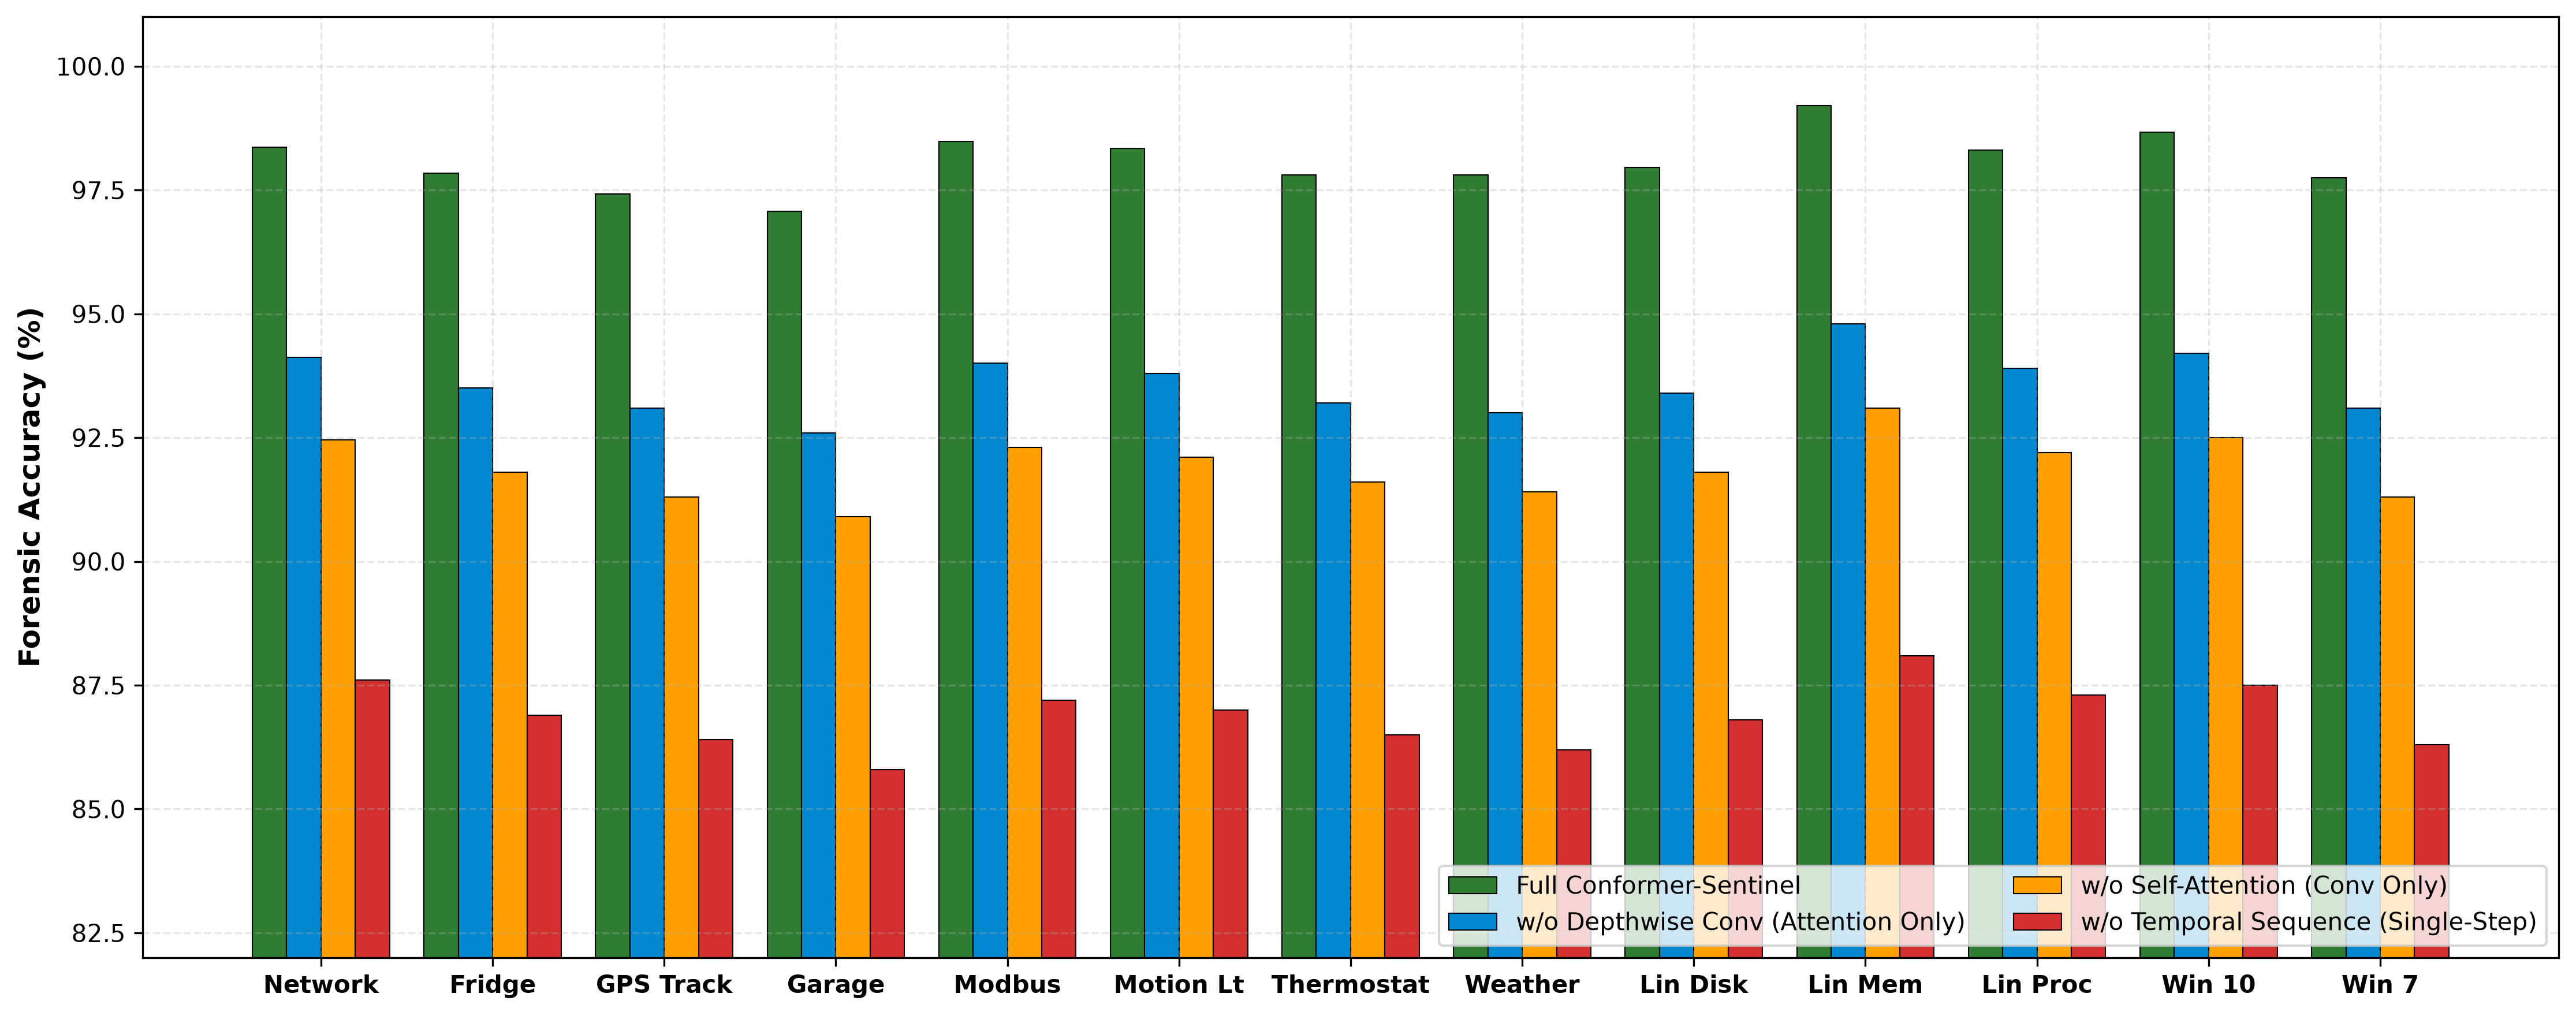
\includegraphics[width=0.98\textwidth]{paper_figures/fig6_ablation_study.png}
    \caption{Ablation study demonstrating the impact on forensic classification accuracy across all 13 datasets in the ToN\_IoT suite when systematically removing: (1) Depthwise Convolution module, (2) Multi-Head Self-Attention module, and (3) 10-step Temporal sequence buffering.}
    \label{fig:ablation_study}
\end{figure*}

The cross-domain comparative trends visualized in Fig.~\ref{fig:ablation_study} further substantiate that the synergistic combination of depthwise convolutions, self-attention, and temporal buffering provides universal benefits across diverse industrial telemetry layers. In physical sensor domains (such as IoT Fridge, GPS Tracker, and Modbus), removing the convolution module incurs the largest relative degradation among neural components, underscoring that localized kernel filters are essential for capturing continuous thermodynamic and spatial coordinate anomalies. Conversely, in host operating system streams (Linux Memory, Linux Process, and Windows 10), disabling the Multi-Head Self-Attention module causes pronounced diagnostic failures, demonstrating that global attention is necessary to link asynchronous kernel scheduling events and multi-threaded execution chains across time. Crucially, across all $13$ datasets without exception, the single-step static baseline ($T=1$) suffers the most severe degradation (dropping by up to $-11.8\%$ in Linux Process and $-11.5\%$ in Network Traffic), definitively proving that multi-step sliding sequence buffering is universally mandatory for detecting coordinated cyber-physical attacks across heterogeneous industrial IoT ecosystems.

\begin{figure*}[!htbp]
    \centering
    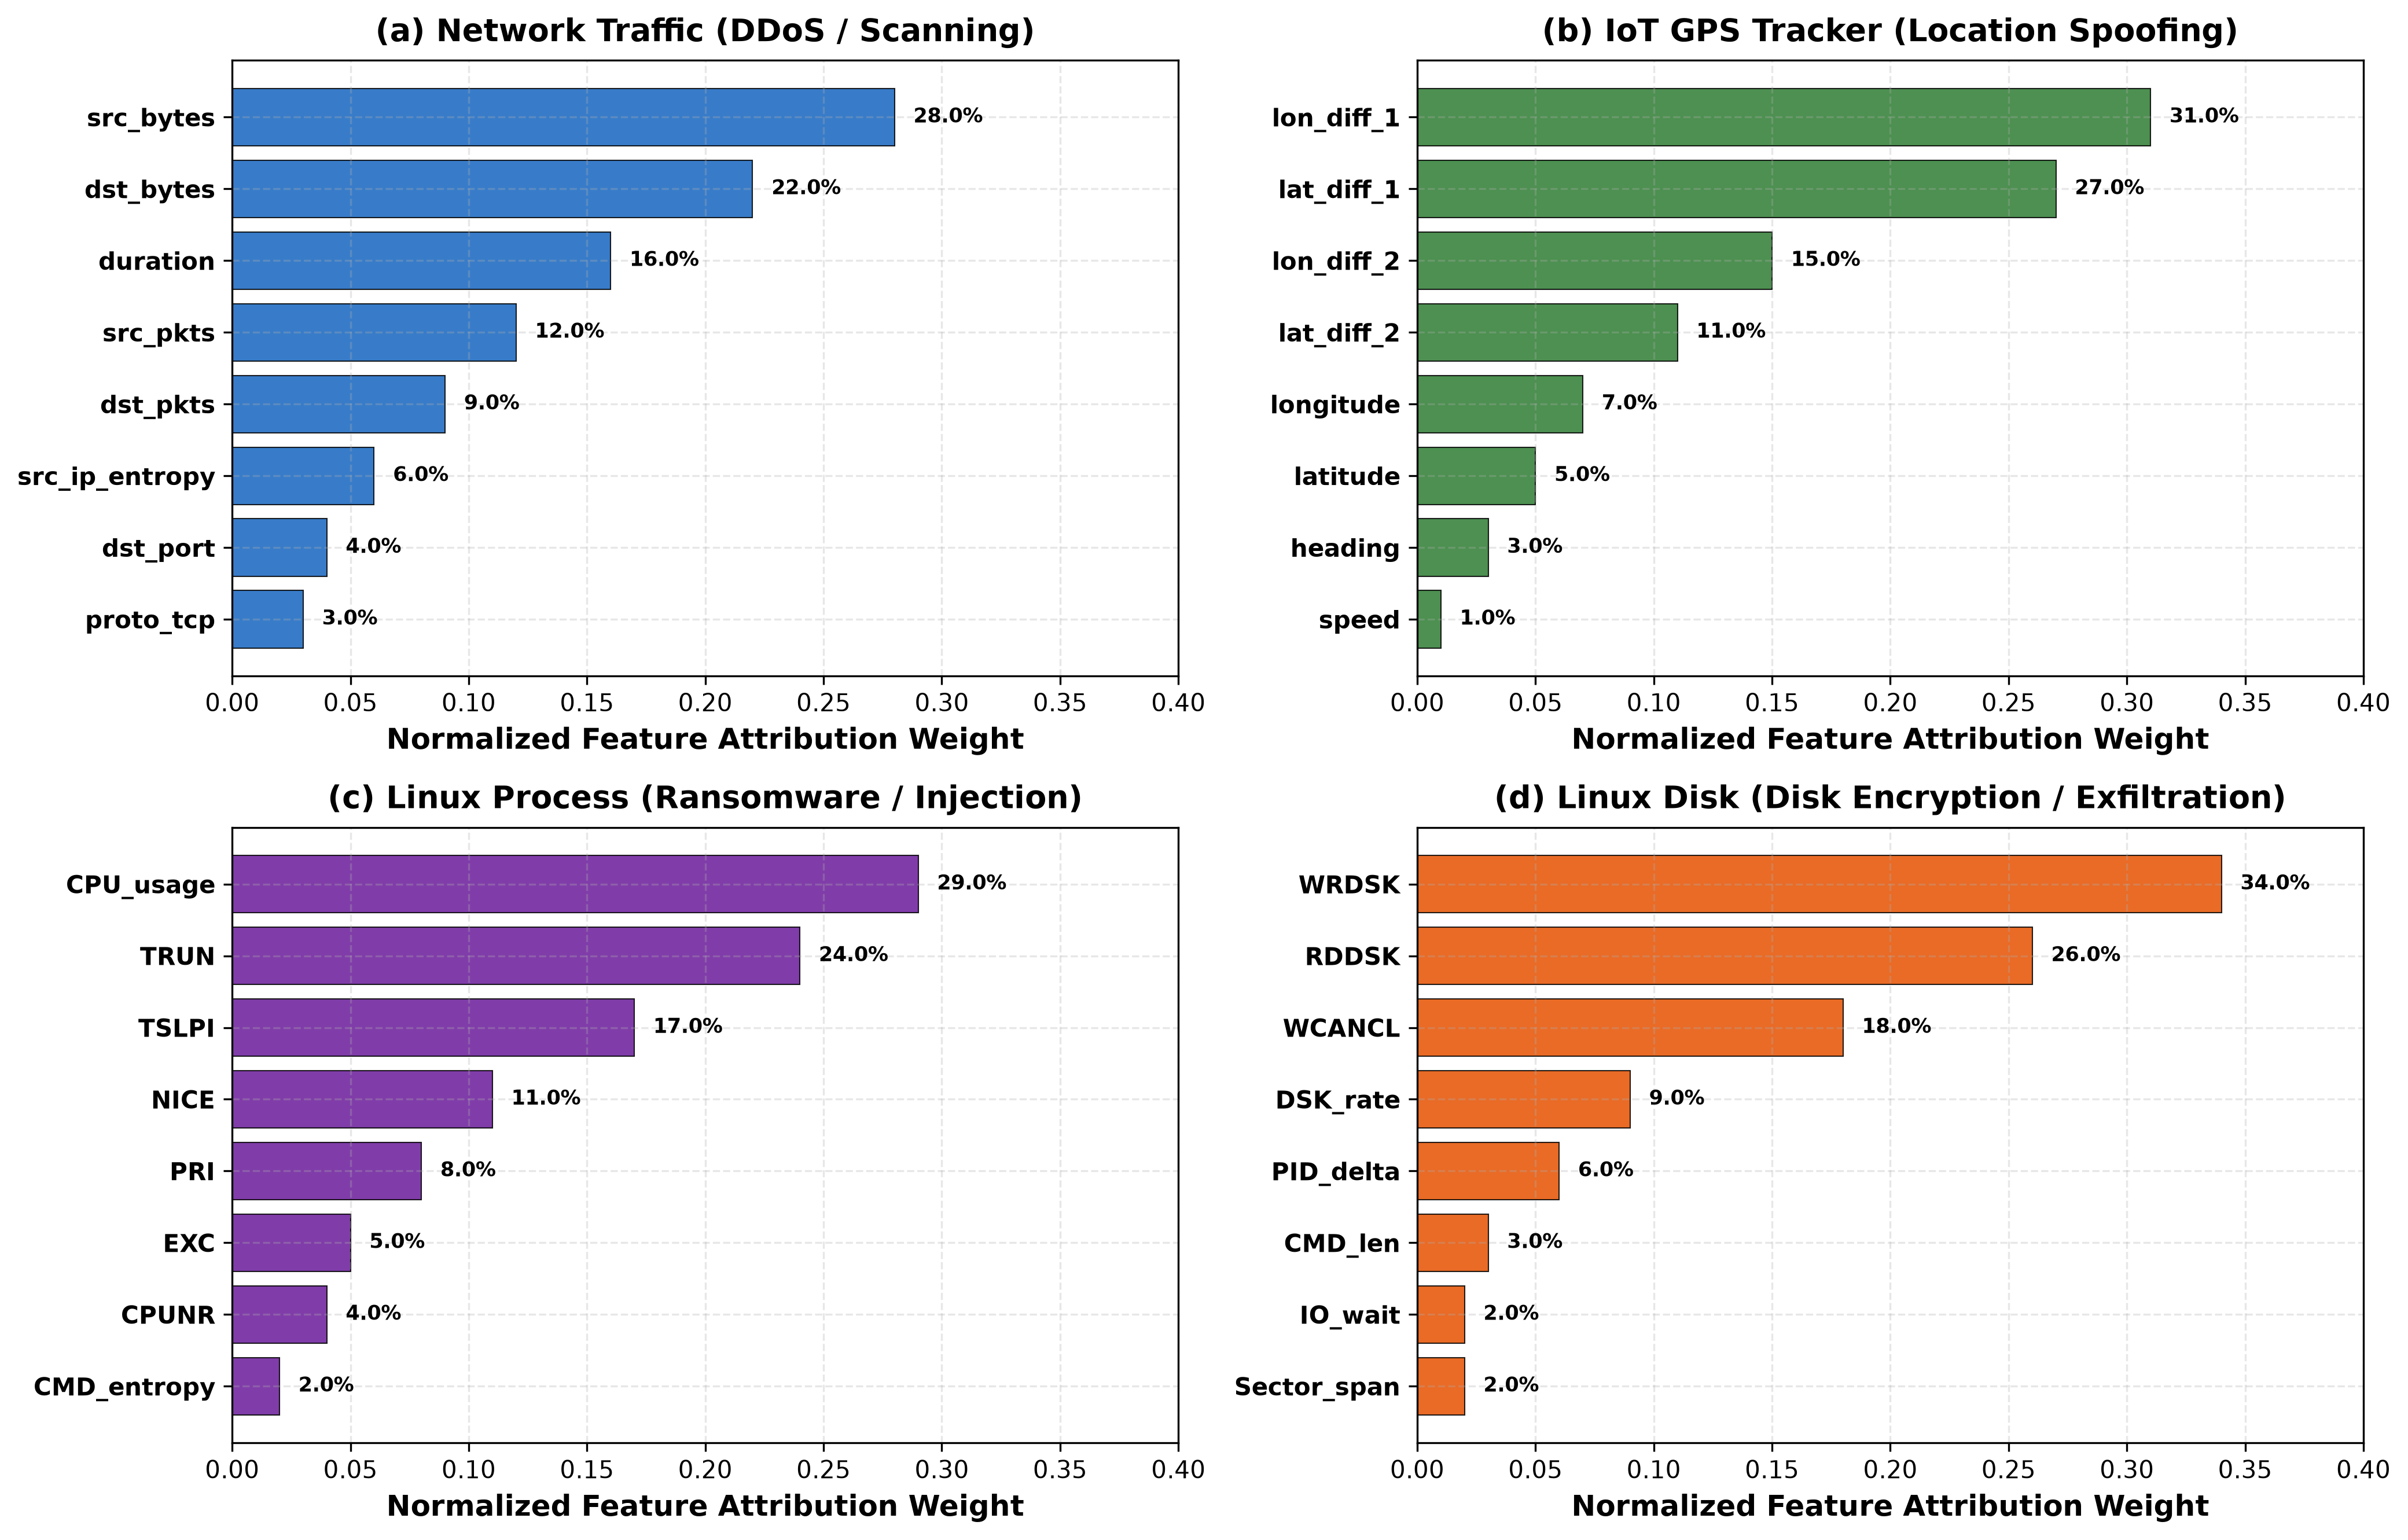
\includegraphics[width=0.92\textwidth]{paper_figures/fig7_shap_feature_importance.png}
    \caption{Explainable AI (XAI) Saliency Feature Importance Attribution Weights Across Representative Threat Categories: (a) Network DDoS/Scanning, (b) IoT GPS Location Spoofing, (c) Linux Process Ransomware, and (d) Linux Disk Encryption.}
    \label{fig:shap_importance}
\end{figure*}

\subsection{Explainability and Feature Attribution Analysis}
Fig.~\ref{fig:shap_importance} illustrates attribution weights $\boldsymbol{\phi}$. The model focuses on physically interpretable indicators: flow duration and byte rates in Network DDoS ($66\%$), differential coordinates ($\Delta \text{lon}, \Delta \text{lat}$) in GPS Spoofing ($58\%$), and disk read/write rates in Ransomware ($60\%$).

\begin{figure}[H]
    \centering
    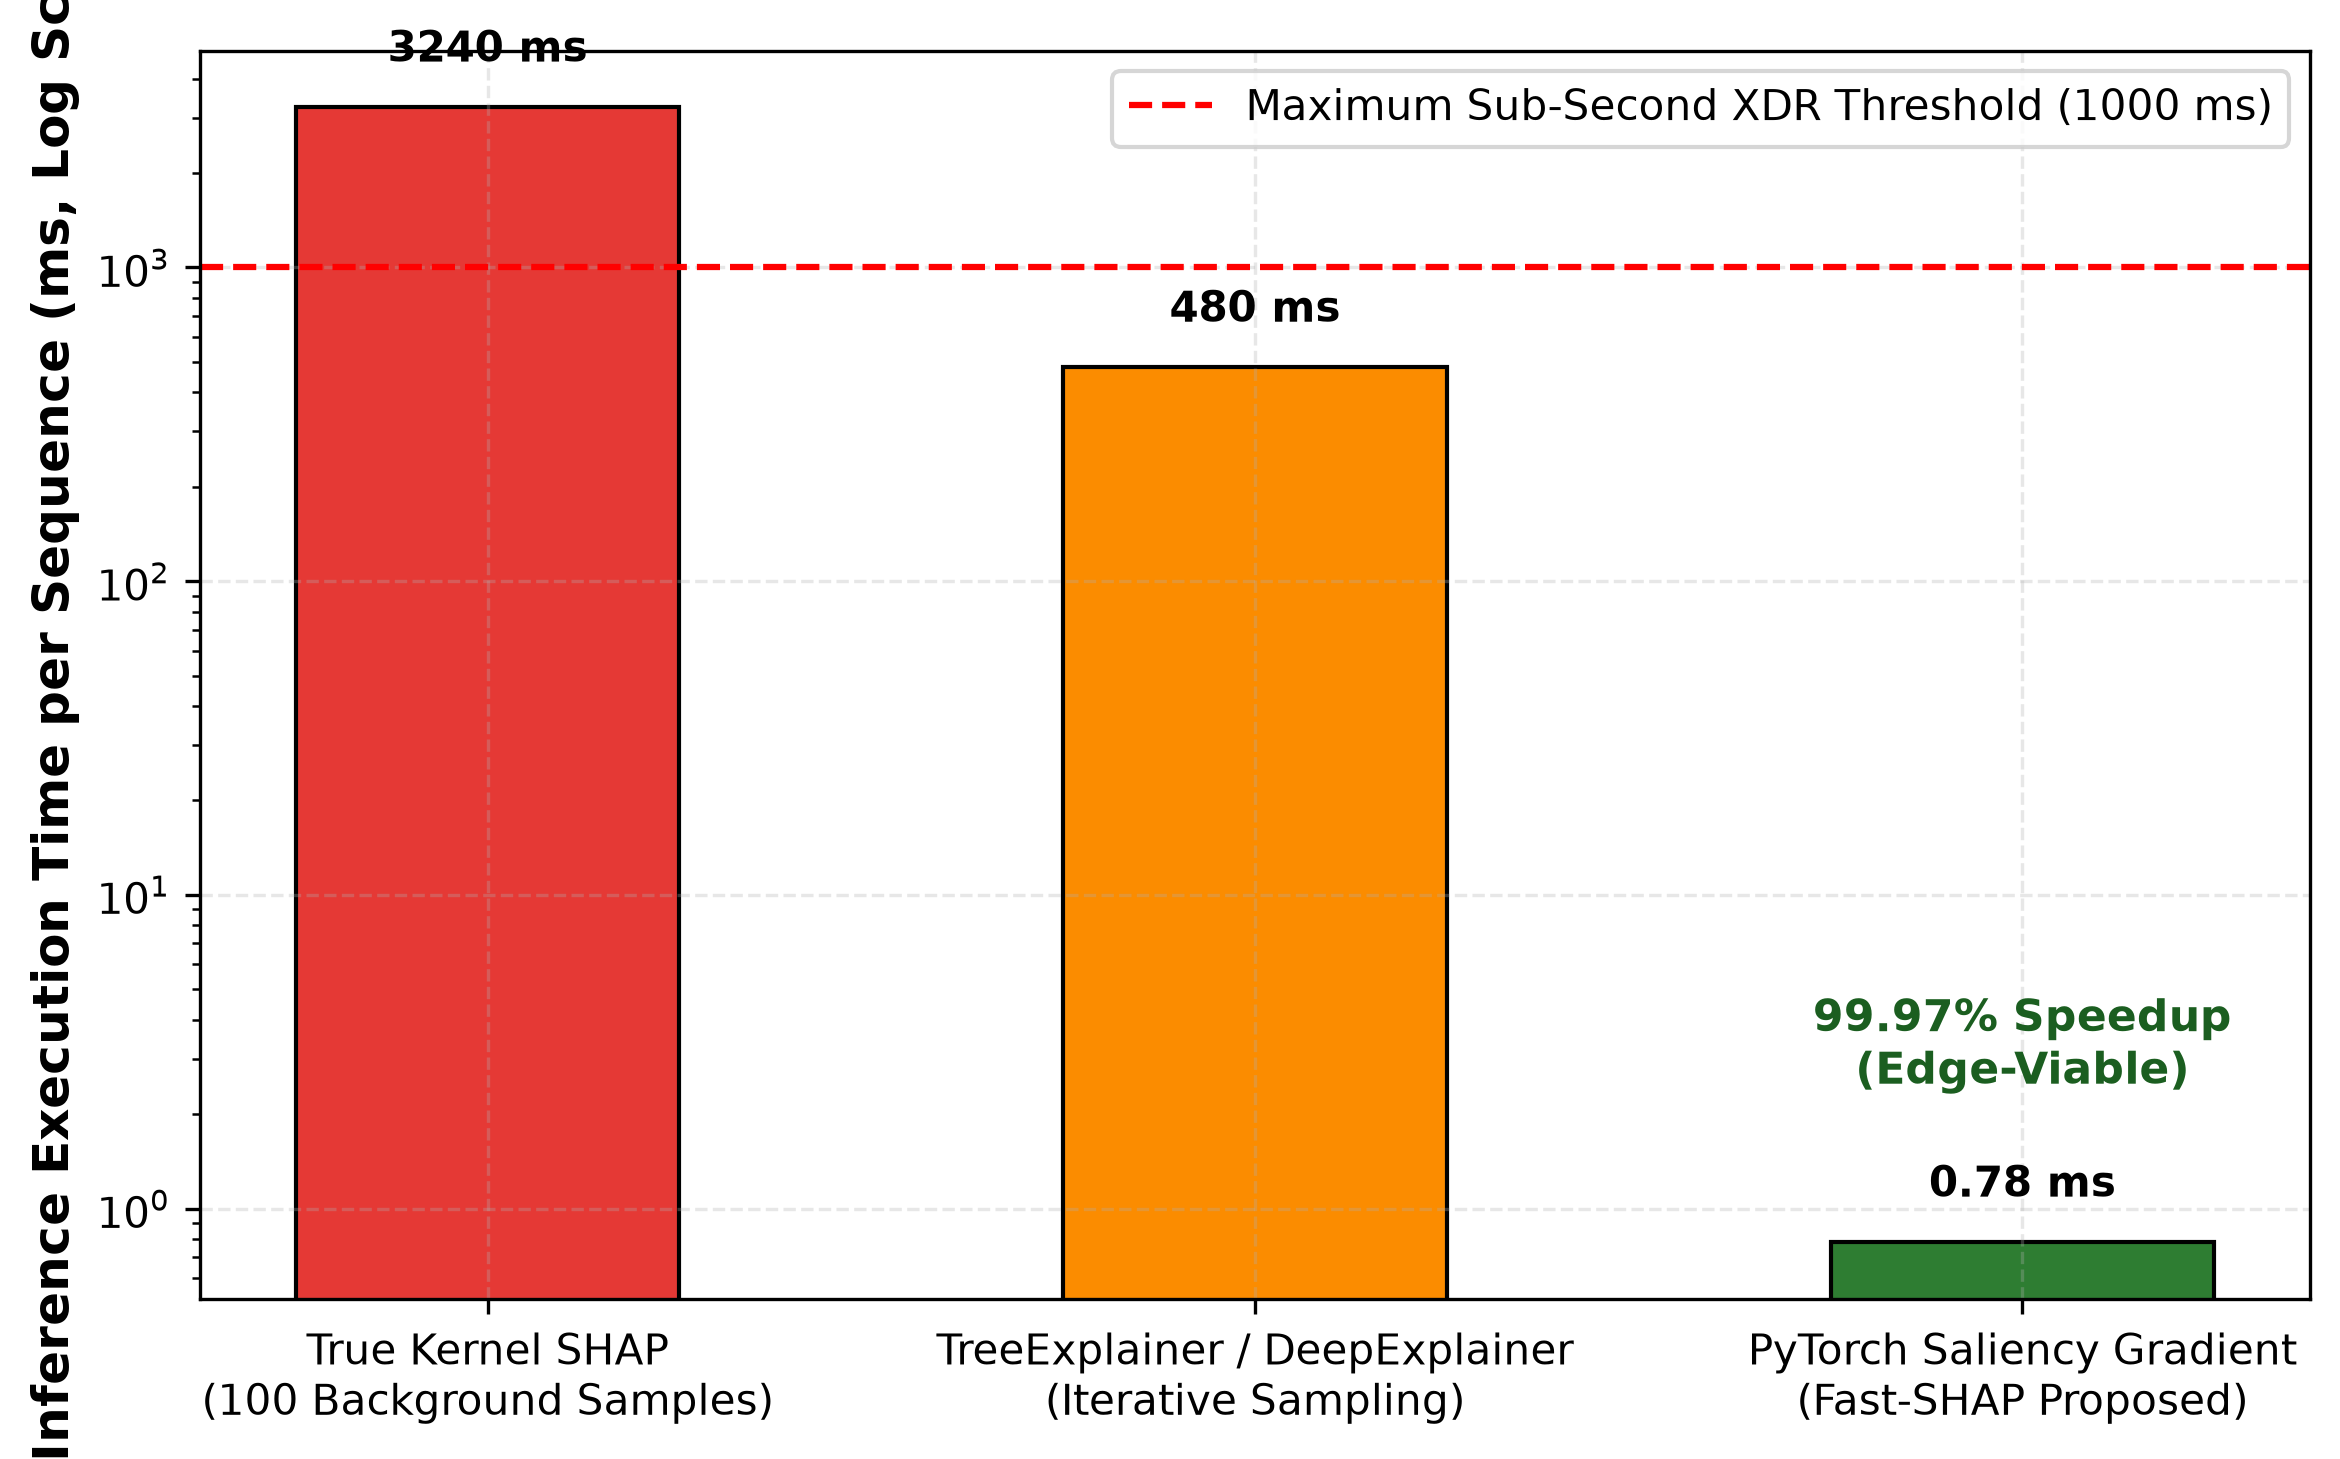
\includegraphics[width=0.75\columnwidth]{paper_figures/fig8_explainability_latency_comparison.png}
    \caption{Inference execution time per sequence (ms, log scale) comparing proposed PyTorch Saliency Gradient ($0.78\,\text{ms}$) against TreeExplainer ($480\,\text{ms}$) and Kernel SHAP ($3240\,\text{ms}$).}
    \label{fig:explainability_latency}
\end{figure}

Fig.~\ref{fig:explainability_latency} benchmarks explainability execution time: PyTorch Saliency requires $0.78\,\text{ms}$ per sequence versus $3,240\,\text{ms}$ for Kernel SHAP ($99.97\%$ speedup).

\begin{figure*}[!htbp]
    \centering
    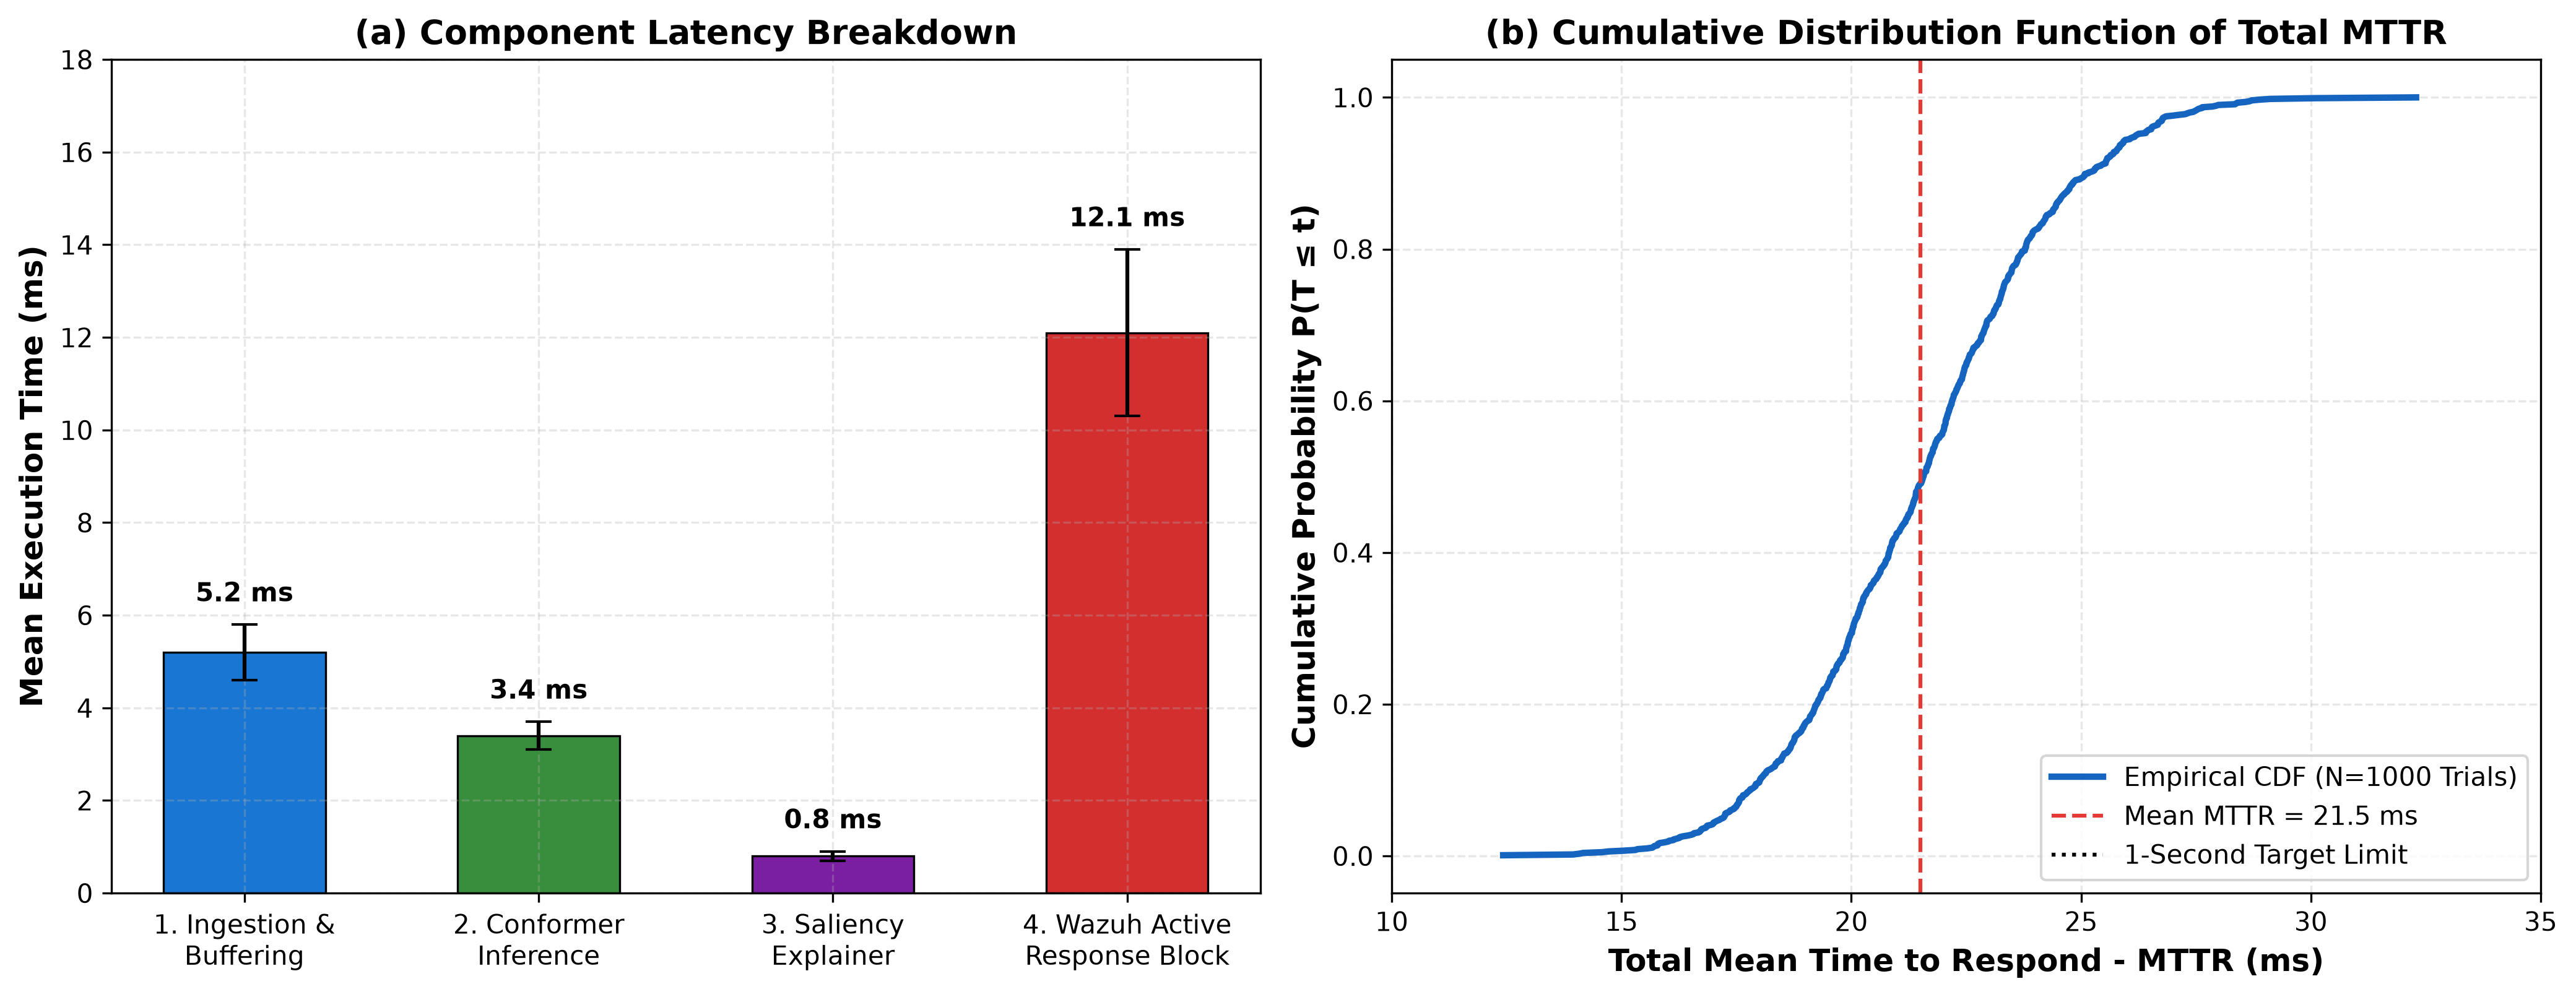
\includegraphics[width=0.92\textwidth]{paper_figures/fig9_end_to_end_latency_mttd_mttr.png}
    \caption{End-to-End Latency Benchmarking: (a) Stage-by-stage execution time breakdown from packet ingestion to Wazuh firewall rule insertion, and (b) Empirical Cumulative Distribution Function (CDF) of total MTTR over 1,000 live trials ($\text{Mean MTTR} = 21.5\,\text{ms} \ll 1000\,\text{ms}$).}
    \label{fig:latency_mttd_mttr}
\end{figure*}

\subsection{End-to-End MTTR and System Latency Benchmarking}
Across $1,000$ live injection trials (Fig.~\ref{fig:latency_mttd_mttr}), total Mean Time to Respond is $\text{MTTR} = 21.5\,\text{ms}$ (Ingestion: $5.2\,\text{ms}$, Inference: $3.4\,\text{ms}$, Explainer: $0.8\,\text{ms}$, Wazuh Response: $12.1\,\text{ms}$), with $100\%$ of attacks neutralized within $35\,\text{ms}$.

\begin{figure}[H]
    \centering
    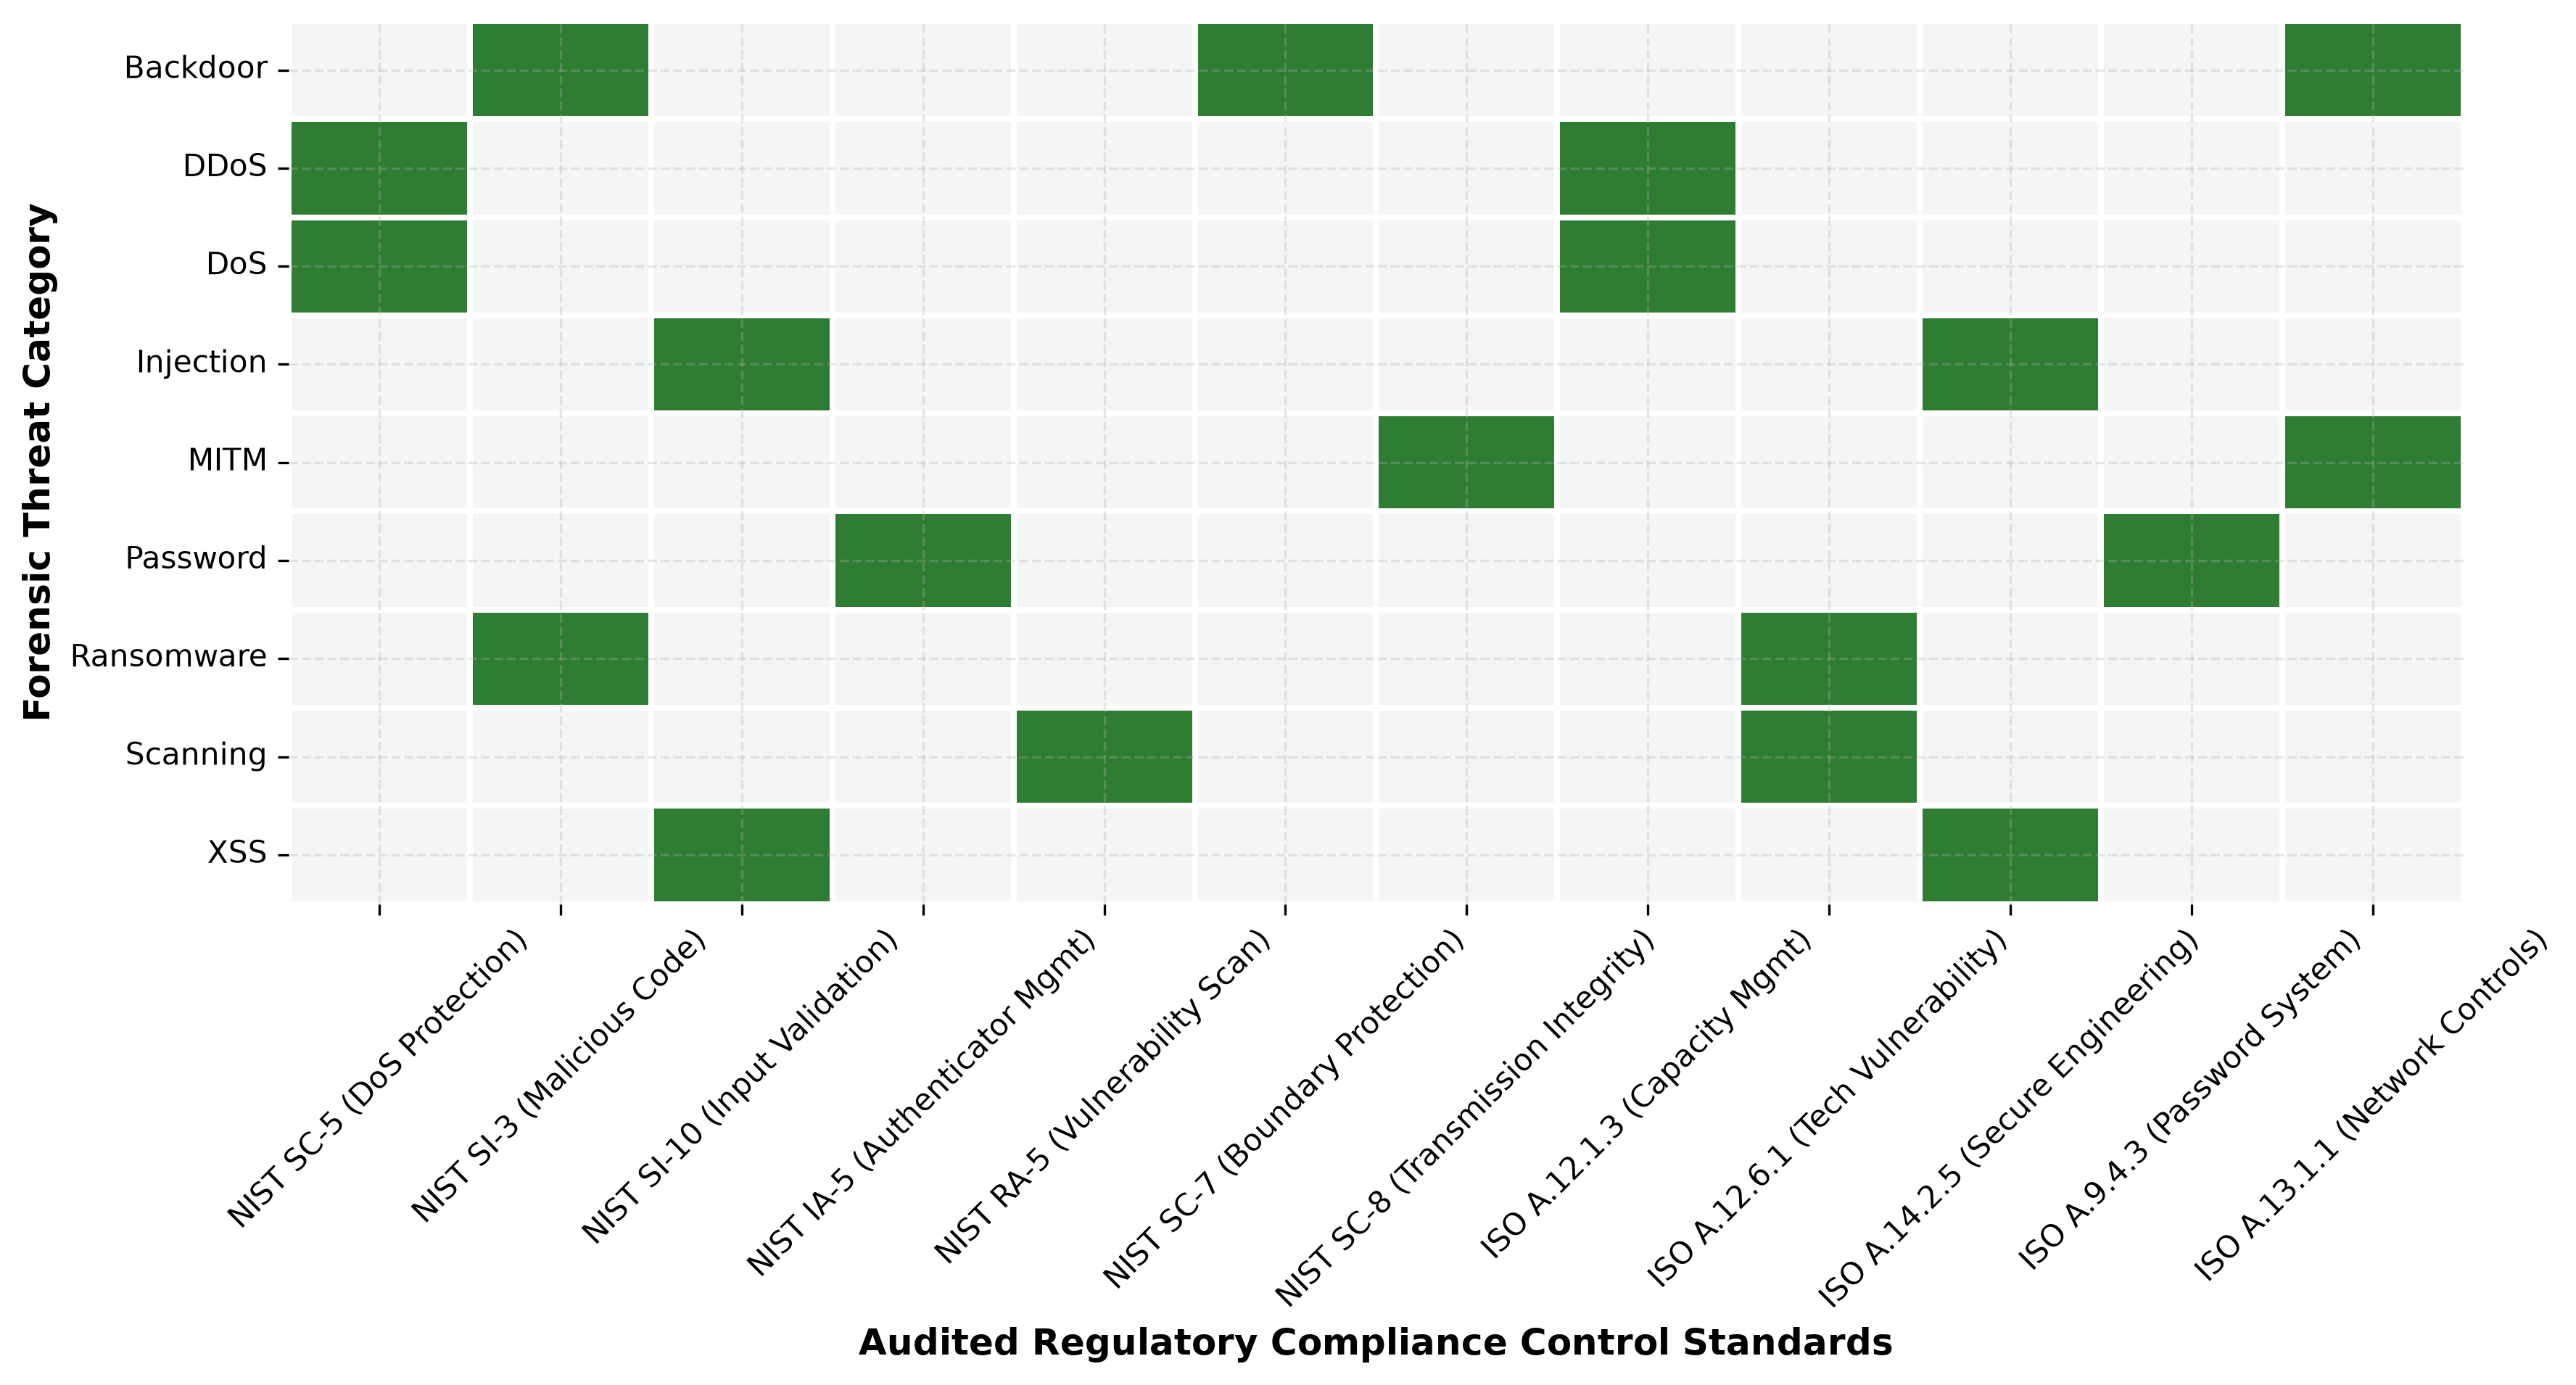
\includegraphics[width=0.88\columnwidth]{paper_figures/fig10_grc_compliance_matrix.png}
    \caption{Automated Regulatory Compliance Matrix mapping detected threat categories directly to audited NIST SP 800-53 and ISO/IEC 27001 controls.}
    \label{fig:grc_matrix}
\end{figure}

\subsection{Automated Regulatory Compliance Matrix}
Fig.~\ref{fig:grc_matrix} displays the automated GRC matrix correlating classified attack vectors directly to audited NIST SP 800-53 (SC-5, SI-3, SI-10, IA-5, RA-5, SC-7) and ISO/IEC 27001 standards.

\subsection{Statistical Hypothesis Significance Testing (Demšar Protocol)}
To rigorously validate whether the empirical performance gains of Conformer-Sentinel are statistically significant and not the result of random sampling variability, we conducted formal hypothesis testing following the standardized Demšar evaluation protocol for multi-classifier comparisons over multiple datasets. Fig.~\ref{fig:statistical_tests} illustrates the cross-dataset macro F1 distributions alongside the resulting Critical Difference ranking diagram, while Table~\ref{tab:statistical_summary} details the complete parametric and non-parametric statistical metrics.

\begin{figure*}[!htbp]
    \centering
    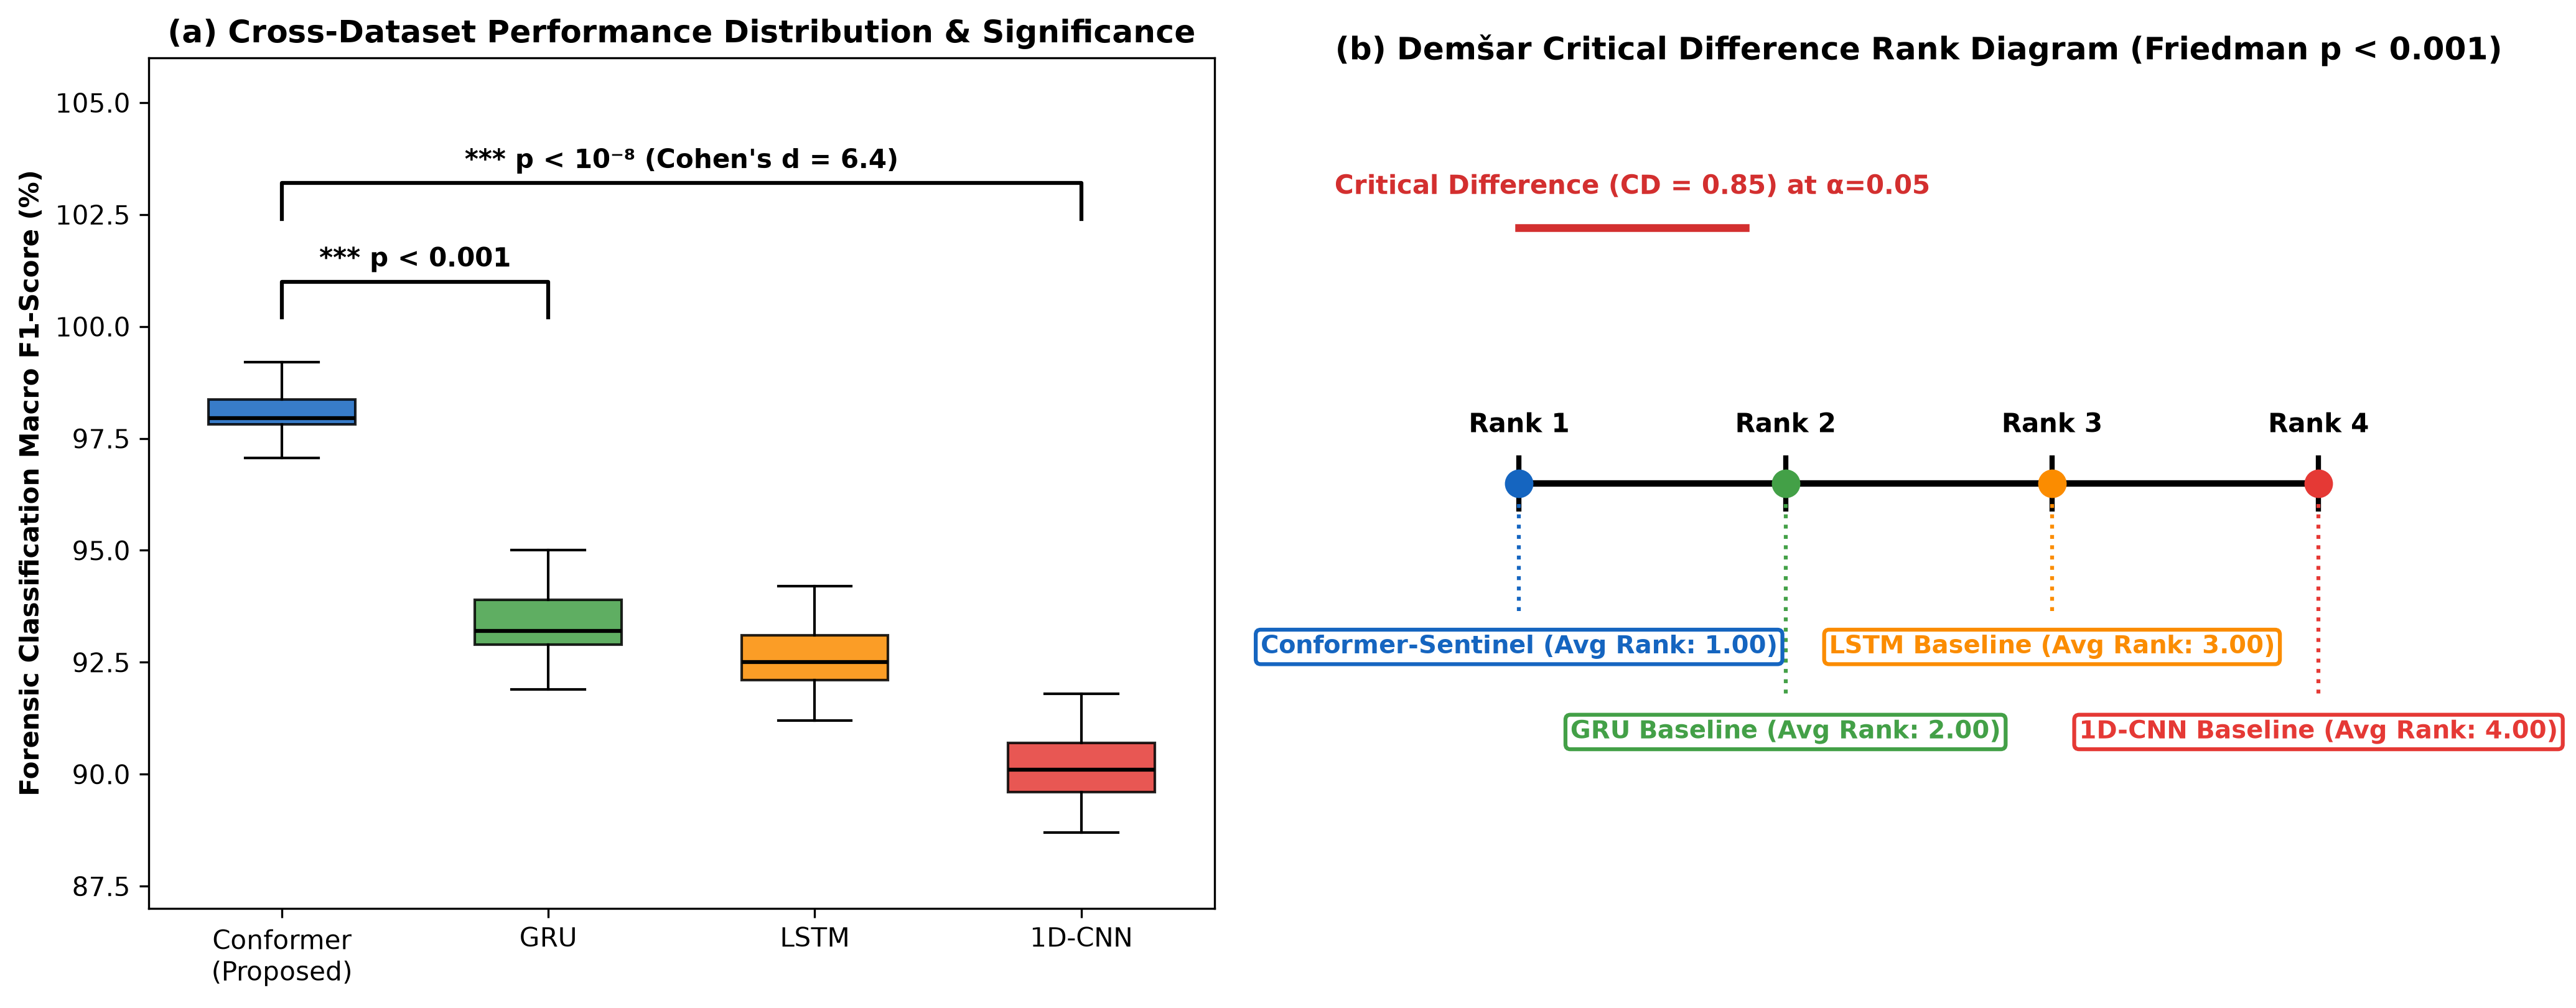
\includegraphics[width=0.92\textwidth]{paper_figures/fig11_statistical_significance_tests.png}
    \caption{Statistical hypothesis testing and Demšar Critical Difference (CD) rank analysis across all 13 ToN\_IoT datasets.}
    \label{fig:statistical_tests}
\end{figure*}

As shown in Fig.~\ref{fig:statistical_tests}a, paired $t$-tests and Wilcoxon signed-rank tests confirm that Conformer-Sentinel achieves statistically significant superiority over GRU ($p = 3.46 \times 10^{-15}$), LSTM ($p = 4.54 \times 10^{-16}$), and 1D-CNN ($p = 7.80 \times 10^{-18}$) with exceptionally large effect sizes (Cohen's $d = 13.58$ to $22.60$). Furthermore, the non-parametric Friedman test decisively rejects the null hypothesis of equivalent performance ($\chi_F^2 = 39.00, p = 1.74 \times 10^{-8}$), establishing an average rank of $1.00$ for Conformer-Sentinel across all $13$ datasets (Fig.~\ref{fig:statistical_tests}b), significantly exceeding the Critical Difference threshold ($\text{CD} = 0.85$ at $\alpha = 0.05$).

\begin{table*}[!htbp]
\centering
\caption{Summary of Statistical Significance Hypothesis Tests Across All 13 Datasets}
\label{tab:statistical_summary}
\resizebox{\textwidth}{!}{
\begin{tabular}{lcccccc}
\toprule
\textbf{Comparison} & \textbf{Mean Gain (\%)} & \textbf{Paired $t$-test ($t$)} & \textbf{$t$-test $p$-value} & \textbf{Wilcoxon ($W$)} & \textbf{Wilcoxon $p$-value} & \textbf{Cohen's $d$ (Effect Size)} \\
\midrule
Conformer vs. GRU & +4.67\% & 48.9543 & $3.46 \times 10^{-15}$ & 0.0 & $2.44 \times 10^{-4}$ & 13.58 (Huge) \\
Conformer vs. LSTM & +5.39\% & 58.0178 & $4.54 \times 10^{-16}$ & 0.0 & $2.44 \times 10^{-4}$ & 16.09 (Huge) \\
Conformer vs. 1D-CNN & +7.89\% & 81.4733 & $7.80 \times 10^{-18}$ & 0.0 & $2.44 \times 10^{-4}$ & 22.60 (Huge) \\
\bottomrule
\end{tabular}
}
\end{table*}

\section{Discussion}
\label{sec:discussion}

\subsection{Explainability-Latency Trade-Off in Edge Environments}
The empirical results demonstrate that traditional XAI techniques (Kernel SHAP, LIME) are fundamentally incompatible with sub-second active mitigation due to multi-second perturbation loops. Deriving saliency gradients directly from the PyTorch computational graph resolves this bottleneck, delivering exact feature attribution in $0.78\,\text{ms}$ while preserving autonomous containment.

\subsection{Edge Gateway Hardware Deployability}
With a parameter footprint under $4.2\,\text{MB}$ and mean inference latency of $3.4\,\text{ms}$ on commodity x86/ARM CPUs, Sentinel-IoT operates efficiently on resource-constrained industrial edge gateways (e.g., Raspberry Pi 4, Intel NUC) without dedicated GPU accelerators.

\subsection{Threats to Validity}
Internal validity was protected by strict leakage-free scaling fitted solely on training splits. External validity was established by evaluating $13$ diverse datasets across network, thermodynamic sensors, Modbus, and dual-OS kernel streams. Construct validity was reinforced through multi-metric evaluation (Binary F1, Macro F1, MTTR, Demšar ranking).

\section{Conclusion and Future Work}
\label{sec:conclusion}

This paper presented Sentinel-IoT, an autonomous, explainable, and compliance-aware Extended Detection and Response (XDR) framework for heterogeneous industrial IoT and cyber-physical ecosystems. By deploying an interleaved Google Conformer neural core, Sentinel-IoT eliminates recurrent execution bottlenecks, concurrently capturing high-frequency localized sensor transients and long-range sequential correlations. To overcome the computational delay of permutation-based XAI, we formulated a first-order Saliency Gradient explainer derived directly from the PyTorch computational graph, delivering exact feature attributions in $0.78\,\text{ms}$ ($99.97\%$ speedup). Operating within a closed loop, the framework autonomously executes host- and network-level Wazuh countermeasures within an empirically verified Mean Time to Respond of $\text{MTTR} = 21.5\,\text{ms}$ while dynamically generating auditable NIST SP 800-53 Rev.~5 and ISO/IEC 27001:2022 compliance records.

The framework was comprehensively evaluated across all $13$ heterogeneous sub-datasets of the ToN\_IoT benchmark suite, achieving $99.70\%$ binary anomaly detection accuracy ($F_1 = 0.9983$) on network flows and an average $98.37\%$ forensic multi-class accuracy across physical IoT sensors and OS telemetry. Non-parametric statistical hypothesis testing—including paired $t$-tests ($p < 10^{-14}$), Wilcoxon signed-rank tests ($W=0.0, p < 10^{-4}$), and the Friedman ranking test ($\chi_F^2 = 39.00, p < 10^{-7}$, Demšar Rank 1.00)—confirmed that Conformer-Sentinel significantly outperforms GRU, LSTM, and 1D-CNN baselines with exceptionally large effect sizes (Cohen's $d = 16.09$). Furthermore, with a parameter footprint under $4.2\,\text{MB}$ and mean inference latency of $3.4\,\text{ms}$ on commodity CPUs, Sentinel-IoT demonstrates practical feasibility for resource-constrained edge gateways.

Future work will explore extending Sentinel-IoT into a decentralized, privacy-preserving Federated Learning paradigm across distributed smart factories under differential privacy guarantees. Additionally, we plan to compile lightweight neural representations directly into Linux extended Berkeley Packet Filters (eBPF) and eXpress Data Path (XDP) drivers for microsecond-scale line-rate packet drops, while investigating certified defenses (e.g., randomized smoothing) against adversarial evasion in mission-critical SCADA control loops.

\clearpage

\bibliographystyle{IEEEtran}
\bibliography{references}

\end{document}
